\documentclass[14pt,a4paper]{extarticle}
% Portable Cyrillic fonts: retain the original path for pdfLaTeX.
\usepackage{iftex}
\ifPDFTeX
  \usepackage[T2A]{fontenc}
  \usepackage[utf8]{inputenc}
\else
  \usepackage{fontspec}
  \IfFontExistsTF{Times New Roman}
    {\setmainfont{Times New Roman}}
    {\setmainfont{DejaVu Serif}}
  \IfFontExistsTF{Courier New}
    {\setmonofont{Courier New}}
    {\setmonofont{DejaVu Sans Mono}}
\fi
\usepackage[english,russian]{babel}
\usepackage[left=25mm,right=20mm,top=20mm,bottom=20mm]{geometry}
\usepackage{amsmath,amssymb,booktabs,array,longtable}
\usepackage{graphicx}
\graphicspath{{figures/}}
\usepackage{enumitem}
\usepackage{titlesec}
\usepackage[unicode,hidelinks]{hyperref}
\setlength{\parindent}{1.25cm}
\setlength{\emergencystretch}{3em}
\setlist{nosep}
\setcounter{tocdepth}{2}
\newcommand{\Sop}{S}
\newcommand{\Cg}{C_g}
\newcommand{\dd}{\mathrm{d}}
\newcommand{\Rnum}{\mathbb{R}}
\DeclareRobustCommand{\code}[1]{\texttt{\let\savedunderscore\_\def\_{\savedunderscore\allowbreak}#1}}
\newcommand{\emptyfield}[1]
{\par\vspace{5mm}\noindent\textbf{#1}\par\vspace{9mm}}
\newcommand{\pt}[1]{\textbf{#1}\ }

\begin{document}
% Титульный лист по образцу «Отчет по проекту.docx».
% Tempora — шрифт семейства Times с кириллицей, доступный в TeX Live.
\hypersetup{pageanchor=false}
\begin{titlepage}
\newgeometry{left=25.4mm,right=25.4mm,top=25.4mm,bottom=25.4mm}
\ifPDFTeX\fontfamily{Tempora-TLF}\fi\fontsize{14}{16}\selectfont
\setlength{\parindent}{0pt}
\begin{center}
федеральное государственное автономное образовательное учреждение\\
высшего образования\\
\textbf{«Национальный исследовательский университет\\
«Высшая школа экономики»}

\vspace{6mm}
\textbf{Московский институт электроники и математики\\
им. А.\,Н. Тихонова}

\vspace{29mm}
\textbf{Отчет\\по проектной работе}

\vspace{3mm}
\textit{«Методы нахождения решений линейных дифференциальных уравнений второго порядка с переменными коэффициентами»}
\end{center}

\vspace{18mm}
\begin{flushright}
{\fontsize{12}{14}\selectfont\textbf{Выполнили студенты}}
\end{flushright}
\vspace{3mm}
{\fontsize{12}{15}\selectfont
\newcommand{\studentfield}[1]{%
\begin{minipage}[t]{0.47\textwidth}
\raggedleft
#1\par
\vspace{4mm}
\rule{45mm}{0.4pt}\\[-1mm]
\textit{(подпись)}
\end{minipage}}
\noindent
\studentfield{Авдеев Евгений Владимирович, БПМ233}\hfill
\studentfield{Евсеев Кирилл Александрович, БПМ231}\par
\vspace{8mm}
\noindent
\studentfield{Тимофеев Михаил Юрьевич, БПМ231}\par
}

\vspace{13mm}
\textbf{Руководитель проекта:}\par
\vspace{6mm}
Парусникова Анастасия Владимировна\par
\vspace{5mm}
\rule{55mm}{0.4pt}\\[-1mm]
{\fontsize{12}{14}\selectfont\textit{(подпись)}}

\vfill
\begin{center}Москва, 2026\end{center}
\end{titlepage}
\hypersetup{pageanchor=true}
\restoregeometry

\section*{Информация о составе проектной команды и контакты}
\phantomsection
\addcontentsline{toc}{section}{Информация о составе проектной команды и контакты}

\subsection*{Парусникова Анастасия Владимировна:}
\textbf{Роль:} руководитель проекта\\
\textbf{Контакты:} aparusnikova@hse.ru
\subsection*{Авдеев Евгений Владимирович}
\textbf{Роль:} научный работник-исследователь\\
\textbf{Контакты:} evavdeev@edu.hse.ru
\subsection*{Евсеев Кирилл Александрович}
\textbf{Роль:} научный работник-исследователь\\
\textbf{Контакты:} kaevseev@edu.hse.ru
\subsection*{Тимофеев Михаил Юрьевич}
\textbf{Роль:} промпт-инженер\\
\textbf{Контакты:} mitimofeev@edu.hse.ru
\clearpage

\section*{Реферат}
\phantomsection
\addcontentsline{toc}{section}{Реферат}
\subsection*{Выбор численного метода с помощью машинного обучения}
\begingroup
\titlespacing*{\subsubsection}{0pt}{5pt}{2pt}
\subsubsection*{Задача}
Рассматривается уравнение
\[
a(x)f''+b(x)f'+\bigl(c(x)-\lambda\bigr)f=-g(x).
\]
Его решение вычисляется четырьмя численными методами: методом Ремизова,
методом Монте-Карло, методом Рунге--Кутты четвёртого порядка (RK4)
и методом мультипликативного интеграла. В основном эксперименте
все методы сравниваются по ошибке в точке $x=0$:
\[
E_m=\bigl|f_m(0)-f(0)\bigr|,
\]
где $f_m$ --- решение, найденное методом $m$, а $f$ --- точное решение.
Метод достигает точности $\varepsilon=0.05$, если $E_m\le0.05$.

\subsubsection*{Цель работы}
Оценить точность методов при фиксированных настройках и проверить,
можно ли до решения уравнения, только по его коэффициентам и правой
части, предсказать метод с меньшей ошибкой.

\subsubsection*{Методика}
\begin{itemize}
\item Построено 1000 уравнений с известным точным решением: задаются
$a,b,c,\lambda$ и $f$, а $g$ вычисляется подстановкой в уравнение.
Уравнения образуют 200 семейств по 5 уравнений.
\item Каждое уравнение описывается 258 числами (признаками): значения
функций $a$, $b$, $c$, $g$ на сетке, их статистики, границы
коэффициентов, характеристики формул коэффициентов и пять отношений
слагаемых уравнения. Первые 253 признака --- основные, пять отношений
добавлены к ним позже.
\item Для выбора между методами Ремизова и Монте-Карло использованы
модели CatBoost (суммы 120 решающих деревьев) на 253 и на 258
признаках. Модели обучаются на 747 уравнениях (Train), порог выбора
подбирается на 100 (Validation), проверка проводится на 150 (Test);
уравнения одного семейства всегда попадают в одну выборку.
По Validation выбрана модель с 253 признаками; модель с 258 признаками
подробно разобрана как дополнительная.
\item Основной критерий --- средняя избыточная ошибка: на сколько
в среднем ошибка выбранного метода больше ошибки лучшего из двух методов.
\item На 258 признаках и тех же выборках обучена отдельная модель
CatBoost для выбора из трёх методов: Ремизова, Монте-Карло
и мультипликативного интеграла. Во всех моделях лучший метод
определяется по ошибке в точке $x=0$.
\item Отдельно по уже сохранённым ответам вычислена наибольшая ошибка
методов Ремизова, RK4 и мультипликативного интеграла по 33 узлам
отрезка $[-1,1]$. Для Монте-Карло сохранено только значение в точке
$x=0$, поэтому его ошибка в нуле использована как оценка снизу.
\item На 60 уравнениях вне тестовой выборки проведён небольшой
эксперимент по времени счёта: для RK4 и мультипликативного интеграла
при числе шагов $N=32,64,128,256$ измерено время расчёта и проверено,
достигается ли наибольшая ошибка в 33 узлах не больше $0.01$ (каждый
вариант запускался один раз пробно и пять раз с измерением времени).
\item На 52 уравнениях вне тестовой выборки для метода Ремизова
сравнены два способа продолжения функции за край окна --- исходный
(с плавным затуханием) и продолжение нулём --- при неизменных
остальных параметрах.
\end{itemize}

\subsubsection*{Результат 1. Методы Ремизова и Монте-Карло}
На 997 уравнениях (для трёх нет сохранённого ответа метода Ремизова)
метод Ремизова точнее в 881 случае, Монте-Карло --- в 116. При этом
у метода Ремизова встречаются редкие очень большие ошибки (до 842),
а ошибка Монте-Карло не превышает $0.57$.

\subsubsection*{Результат 2. Модели выбора из двух методов}
Выбранная по Validation модель с 253 признаками на Test дала
91.33\% верных выборов, а выбранный ею метод достиг точности $0.05$
на 146 из 150 уравнений. Модель с 258 признаками нашла 6 из 9 уравнений,
где точнее Монте-Карло, но 14 раз выбрала Монте-Карло ошибочно; в двух
случаях из-за этого ошибка превысила $0.05$. Малая средняя ошибка этой
модели объясняется в основном одним уравнением, где ошибка метода
Ремизова равна 248. Без этого уравнения постоянный выбор метода
Ремизова даёт меньшую среднюю ошибку, чем эта модель.

\subsubsection*{Результат 3. Четыре метода}
RK4 даёт наименьшую ошибку в точке $x=0$ на всех 997 уравнениях
и достигает точности $0.05$ на всех 1000. Поэтому на этом наборе выбор
из четырёх методов тривиален, и модель для него не обучалась.

\subsubsection*{Результат 4. Выбор из трёх методов}
Без RK4 лучшие методы распределены так: на 826 уравнениях точнее
остальных двух метод Ремизова, на 106 --- Монте-Карло, на 65 --- метод
мультипликативного интеграла. Модель верно определила лучший метод на 133 из 150
тестовых уравнений (88.67\%), а выбранный ею метод достиг точности $0.05$
на 147 (98\%). Однако постоянный выбор метода Ремизова верен на 136
уравнениях (90.67\%) и тоже достигает точности на 147, поэтому
преимущества у модели нет.

\subsubsection*{Результат 5. Проверка по 33 узлам}
По наибольшей ошибке в 33 узлах отрезка $[-1,1]$ точность $0.05$
достигается у метода Ремизова на 970 из 997 уравнений, у RK4 --- на 1000
из 1000, у мультипликативного интеграла --- на 404 из 1000. На всех
997 общих уравнениях ошибка RK4 меньше, чем у методов Ремизова
и мультипликативного интеграла, и даже меньше ошибки Монте-Карло
в одной точке $x=0$. Поэтому RK4 остаётся самым точным и по 33 узлам.
Ошибка Монте-Карло во всех 33 узлах не вычислялась; оценки наибольшей
ошибки на всём отрезке (а не только в узлах) нет.

\subsubsection*{Результат 6. Время счёта при заданной точности}
Требовалось, чтобы наибольшая ошибка в 33 узлах была не больше $0.01$.
Если для каждого уравнения выбирать самый быстрый вариант, достигающий
этой точности (идеальный выбор по уже известным ошибкам и временам), то
всегда выбирается RK4: 59 раз с $N=32$ и один раз с $N=64$. Лучший
единый для всех уравнений вариант --- RK4 с $N=64$. Идеальный выбор
быстрее его в среднем на 49.2\% (по сумме времён --- на 48.3\%), но
весь этот выигрыш даёт выбор $N$ внутри RK4: мультипликативный
интеграл ни разу не оказался быстрее. Поэтому обучать модель выбора
между RK4 и мультипликативным интегралом в такой постановке
нецелесообразно. Это оценка возможного выигрыша, а не результат
обученной модели.

\subsubsection*{Результат 7. Продолжение за край окна в методе Ремизова}
При продолжении нулём все три ошибки $E_{33}>1$ стали меньше единицы.
На 30 контрольных уравнениях точность $0.05$ сохранилась на всех 30,
а из 22 уравнений с ошибкой больше $0.05$ точности достигло одно
(раньше ни одного). Заранее заданное строгое условие <<ни одна ошибка
не увеличилась>> не выполнено: в трёх случаях ошибка выросла примерно
на $10^{-9}$, что практически незаметно. Основной вариант расчёта
не заменялся; устойчивость численной схемы по $x$ полностью
не доказана.

\subsubsection*{Выводы}
\begin{enumerate}
\item Метод Ремизова чаще точнее Монте-Карло, но изредка даёт очень
большую ошибку.
\item Выбор более точного из двух методов и достижение точности $0.05$ ---
разные свойства: верно выбранный метод может не достигать точности.
\item Модель с 258 признаками находит часть уравнений, где точнее
Монте-Карло, но ценой многих ошибочных выборов Монте-Карло. Ни
выбранная модель выбора из двух методов, ни модель выбора из трёх
методов не дали на Test устойчивого выигрыша перед постоянным выбором
метода Ремизова.
\item При выбранных настройках и точных начальных условиях RK4
оказался самым точным в точке $x=0$ и остаётся самым точным по 33
узлам. Модели выбора при этом по-прежнему оцениваются только
по ошибке в точке $x=0$.
\item В эксперименте по времени счёта добавление мультипликативного
интеграла к RK4 не даёт выигрыша. Продолжение нулём за край окна
устраняет очень большие ошибки метода Ремизова, но строгое условие
<<ни одна ошибка не увеличилась>> не выполнено. Эти два отрицательных
итога имеют разные причины.
\end{enumerate}
\endgroup
\clearpage
\tableofcontents
\clearpage

\section{Основная часть}
\subsection{Введение}
\subsubsection{Объект и предмет исследования}
Объект исследования --- линейные неоднородные дифференциальные
уравнения второго порядка с переменными коэффициентами. Предмет
исследования --- точность четырёх численных методов их решения (метода
Ремизова, метода Монте-Карло, RK4 и метода мультипликативного интеграла)
и возможность заранее, по коэффициентам уравнения, выбрать метод
с меньшей ошибкой.

\subsubsection{Цель и задачи}
Цель работы --- оценить точность численных методов при фиксированных
настройках и проверить, можно ли до решения уравнения предсказать метод
с меньшей ошибкой.

Для достижения цели решались следующие задачи:
\begin{enumerate}
\item Построить набор из 1000 уравнений с известными точными решениями.
\item Вычислить ошибки четырёх методов в точке $x=0$ при фиксированных
настройках.
\item Описать каждое уравнение набором признаков, которые вычисляются
до его решения.
\item Обучить модель выбора между методами Ремизова и Монте-Карло
и сравнить её с простыми правилами выбора.
\item Разобрать все неверные выборы модели с 258 признаками
на тестовой выборке.
\item Сравнить четыре метода и определить, имеет ли смысл модель выбора
из четырёх методов.
\item Обучить модель выбора из трёх методов --- Ремизова, Монте-Карло
и мультипликативного интеграла --- и сравнить её с постоянным выбором
одного метода.
\item По сохранённым ответам проверить ошибку методов в 33 узлах
отрезка $[-1,1]$ и выяснить, остаётся ли RK4 самым точным, не вычисляя
заново решения методом Монте-Карло.
\item На небольшой выборке уравнений вне Test проверить, сокращает ли
выбор между RK4 и мультипликативным интегралом время счёта при
наибольшей ошибке в 33 узлах не больше $0.01$ по сравнению с лучшим
единым вариантом и с выбором числа шагов только у RK4.
\item На уравнениях вне Test проверить, устраняет ли продолжение нулём
за край окна (вместо плавного затухания) большие ошибки метода
Ремизова, не ухудшая точность на остальных уравнениях; формула метода
и остальные параметры при этом не меняются.
\end{enumerate}

\subsection{Ход работы}
\subsubsection{Математическая постановка}
Рассматривается уравнение
\begin{equation}\label{eq:ode}
a(x)f''(x)+b(x)f'(x)+\bigl(c(x)-\lambda\bigr)f(x)=-g(x),
\end{equation}
где коэффициенты $a,b,c$, правая часть $g$ и число $\lambda$ заданы,
а $f$ --- искомое решение.

Методы Ремизова и Монте-Карло решают уравнение~\eqref{eq:ode} на всей
прямой и начальных условий не используют. RK4 и метод мультипликативного
интеграла решают задачу Коши на отрезке $[-1,1]$ с начальными условиями
$f(-1)$ и $f'(-1)$, сохранёнными при построении уравнения. Для нового
уравнения, точное решение которого неизвестно, такие начальные условия
должны быть известны заранее.

Если записать уравнение~\eqref{eq:ode} в обычном виде
$af''+bf'+\tilde c f=\tilde g$, то $\tilde c=c-\lambda$
и $\tilde g=-g$.

Методы Ремизова и Монте-Карло ищут решение, ограниченное на всей
прямой. Построенная функция $f$ равна нулю вне некоторого отрезка
и по построению удовлетворяет уравнению. При гладких ограниченных
коэффициентах, $\inf_x a(x)>0$ и $\lambda-C>0$ ограниченное решение
единственно, поэтому оно совпадает с $f$. Начальные условия задачи
Коши взяты из той же функции, а решение задачи Коши единственно;
значит, все четыре метода приближают одну и ту же функцию $f$. Однако
RK4 и мультипликативный интеграл дополнительно получают точные значения
$f(-1)$ и $f'(-1)$. Поэтому исходные данные у методов разные, и объём
вычислений у них тоже не одинаков.

В основном эксперименте методы сравниваются по ошибке в одной точке $x=0$:
\begin{equation}\label{eq:ml-error}
E_m=\bigl|f_m(0)-f(0)\bigr|,
\end{equation}
где $m$ --- метод, $f_m$ --- найденное им решение, $f$ --- точное
решение. Будем говорить, что метод достигает точности $\varepsilon$,
если $E_m\le\varepsilon$; принят порог $\varepsilon=0.05$. Лучшим считается
метод с наименьшей ошибкой $E_m$. Лучший метод не обязательно достигает
точности $\varepsilon$: ошибки обоих сравниваемых методов могут быть
больше $0.05$.

\subsubsection{Набор уравнений}
Уравнения строятся методом подставленного решения: сначала задаётся
точное решение $f$ --- гладкая функция, равная нулю вне некоторого
отрезка, затем правая часть $g$ вычисляется подстановкой $f$
в уравнение~\eqref{eq:ode}. Коэффициенты задаются формулами
\begin{equation}\label{eq:ml-coef}
\begin{gathered}
a=A_{\mathrm{mid}}+A_{\mathrm{half}}\tanh T_a(x),\qquad
b=B\tanh T_b(x),\\
c=C\tanh T_c(x),\qquad
\lambda=C+\delta,
\end{gathered}
\end{equation}
где $T_a,T_b,T_c$ --- формулы, составленные из элементарных функций
(виды операций перечислены в приложении, раздел П.4),
$0<A_{\mathrm{half}}<A_{\mathrm{mid}}$ и $\delta>0$. Поскольку
$|\tanh u|<1$, при всех $x$ выполняются оценки
\[
0<A_-\le a(x)\le A_+,\qquad |b(x)|\le B,\qquad |c(x)|\le C,\qquad
\lambda-C=\delta>0,
\]
где $A_\pm=A_{\mathrm{mid}}\pm A_{\mathrm{half}}$. Тем самым коэффициент
$a$ положителен и $\lambda>\sup_x|c(x)|$ на всей прямой.
Для обоснования формул, на которых основаны методы Ремизова
и Монте-Карло, одних этих неравенств недостаточно. В данном наборе
коэффициенты, кроме того, гладкие и ограничены вместе со своими
производными, а точное решение и правая часть равны нулю вне некоторого
отрезка. При этом теоретические свойства формул не гарантируют точности
их численной реализации на конечном окне с интерполяцией.

Набор содержит 1000 уравнений: 200 семейств по 5 уравнений. Семейство ---
это формулы одного вида с разными числовыми параметрами. Уравнения
разделены на четыре уровня сложности L1--L4 (по 250 уравнений) и на пять
режимов поведения коэффициентов (по 200 уравнений): постоянные, медленно
меняющиеся, умеренно меняющиеся, осциллирующие и с большим разбросом
значений.

Для трёх уравнений расчёт методом Ремизова прервался, и ответ
не сохранился; причина не установлена. Эти уравнения не входят
в сравнение, поэтому сравнение методов Ремизова и Монте-Карло
и обучение моделей ведутся на 997 уравнениях. Отсутствие результата не означает, что метод к этим
уравнениям неприменим. Исключены уравнения
\texttt{AMV1\_F0134\_S03}, \texttt{AMV1\_F0136\_S01}
и \texttt{AMV1\_F0139\_S00}.

\subsubsection{Численные методы}\label{sec:ml-methods}
\paragraph{Метод Ремизова\\}
Метод использует оператор
\[
(S(t)\phi)(x)=\tfrac14\phi\bigl(x+2\sqrt{a(x)t}\bigr)
+\tfrac14\phi\bigl(x-2\sqrt{a(x)t}\bigr)
+\tfrac12\phi\bigl(x+2b(x)t\bigr)+t\,c(x)\phi(x).
\]
Приближённое решение при числе композиций $n$ задаётся формулой
\begin{equation}\label{eq:fn}
f_n(x)=\int_0^\infty e^{-\lambda t}\bigl(S(t/n)^ng\bigr)(x)\,\dd t.
\end{equation}
Для вычисления формулы~\eqref{eq:fn} используется следующий алгоритм:
\begin{enumerate}
\item Выбирается окно $[L,R]$, более широкое, чем отрезок $[-1,1]$,
и строится равномерная сетка. На ней вычисляются коэффициенты
и значения $g$.
\item Интеграл по $t$ обрезается на отрезке $[0,T]$, где
\[
T=\max\left(0,\ \frac1\delta\ln\frac{2}{\delta\,\varepsilon_T}\right),
\qquad \delta=\lambda-C,
\]
и выбирается сетка узлов $t_j$ квадратурной формулы по $t$.
Параметр $\varepsilon_T$ задаёт правило выбора $T$, но не равен полной
погрешности. Для формулы~\eqref{eq:fn} без дискретизации отброшенная
часть интеграла оценивается через $\|g\|_\infty=\sup_x|g(x)|$:
\[
\left\|\int_T^\infty e^{-\lambda t}S(t/n)^ng\,\dd t\right\|_\infty
\le\frac{\|g\|_\infty}{\delta}e^{-\delta T}
\le\frac{\|g\|_\infty\varepsilon_T}{2}.
\]
При численном расчёте к этому добавляются ошибки от конечного $n$,
от квадратурной формулы, от интерполяции и от конечного окна.
\item Для каждого узла $t_j$ задаётся $\tau_j=t_j/n$ и $u^{(0)}=g$;
последовательно вычисляются $u^{(k+1)}=S(\tau_j)u^{(k)}$,
$k=0,\dots,n-1$. Значения в сдвинутых точках, не совпадающих с узлами
сетки, восстанавливаются кубическим сплайном. За краем окна сплайн
продолжается по касательной прямой и умножается на множитель,
плавно убывающий до нуля; сами значения при этом не обязательно
становятся малыми.
\item Полученное $u^{(n)}$ умножается на $e^{-\lambda t_j}$, и интеграл
по $t$ приближается по формуле Симпсона.
\end{enumerate}

\paragraph{Метод Монте-Карло\\}
Решение записывается как математическое ожидание (формула
Фейнмана--Каца):
\[
f(x_0)=\mathbb E\int_0^\infty
e^{-\lambda t+\int_0^t c(X_s)\,\dd s}\,g(X_t)\,\dd t,
\]
где $X_t$ --- случайный процесс, заданный уравнением
\[
\dd X=b(X)\,\dd t+\sqrt{2a(X)}\,\dd W,\qquad X_0=x_0,
\]
а $W$ --- винеровский процесс.
Алгоритм:
\begin{enumerate}
\item Интеграл по $t$ обрезается на конечном отрезке $[0,T]$.
\item Из точки $x_0$ запускаются $M$ траекторий по схеме
Эйлера--Маруямы с фактическим шагом $h$:
\[
X_{k+1}=X_k+b(X_k)\,h+\sqrt{2a(X_k)\,h}\;\xi_k,
\]
где $\xi_k$ --- независимые случайные величины с распределением
$\mathcal N(0,1)$.
\item Интеграл $\int_0^tc(X_s)\,\dd s$ в показателе экспоненты и внешний
интеграл по $t$ приближаются по формуле трапеций; для каждой траектории
получается
число $S_j$, $j=1,\dots,M$.
\item $f(x_0)\approx\frac1M\sum_{j=1}^MS_j$.
\end{enumerate}
В работе $x_0=0$. Выполнены четыре независимых расчёта
по $M=1024$ траектории, и используется их среднее:
\[
E_{\mathrm{MC}}=\Bigl|\frac14\sum_{s=1}^4 f_{\mathrm{MC},s}(0)-f(0)\Bigr|.
\]
Это ошибка среднего значения, а не средняя ошибка отдельных расчётов.
Верхний предел $T$ для Монте-Карло выбирается отдельно из условия
$G e^{-\delta T}/\delta\le10^{-4}$, где $G$ --- известная из формул
оценка сверху для $\|g\|_\infty$. Это условие ограничивает только ошибку
от обрезания интеграла, но не случайную ошибку и не ошибку от конечного
шага по времени. Число $\Delta t=1/128$ --- наибольший допустимый шаг:
число шагов $N=\lceil T/\Delta t\rceil$, фактический шаг
$h=T/N\le\Delta t$. Доверительные интервалы метода Монте-Карло
относятся к математическому ожиданию уже обрезанного
и дискретизованного интеграла, поэтому гарантированной оценки полной
ошибки относительно точного решения нет.

\paragraph{Метод Рунге--Кутты (RK4)\\}
Уравнение~\eqref{eq:ode} записывается как система для $Y=(f,v)$, где
$v=f'$:
\[
Y'=F(x,Y),\qquad
F(x,Y)=\Bigl(v,\ \frac{(\lambda-c(x))f-b(x)v-g(x)}{a(x)}\Bigr).
\]
На каждом шаге $h$ вычисляются
\begin{enumerate}
\item $k_1=F(x_k,\ Y_k)$,
\item $k_2=F\bigl(x_k+\tfrac h2,\ Y_k+\tfrac h2k_1\bigr)$,
\item $k_3=F\bigl(x_k+\tfrac h2,\ Y_k+\tfrac h2k_2\bigr)$,
\item $k_4=F(x_k+h,\ Y_k+hk_3)$,
\item $Y_{k+1}=Y_k+\tfrac h6\,(k_1+2k_2+2k_3+k_4)$.
\end{enumerate}
Начальное значение $Y_0=\bigl(f(-1),f'(-1)\bigr)$.

\paragraph{Метод мультипликативного интеграла\\}
Уравнение записывается как система для вектора $Z=(f,f',1)^T$:
\[
Z'=B(x)\,Z,\qquad
B(x)=\begin{pmatrix}
0 & 1 & 0\\[2pt]
\dfrac{\lambda-c}{a} & -\dfrac{b}{a} & -\dfrac{g}{a}\\[8pt]
0 & 0 & 0
\end{pmatrix}.
\]
Шаг делается по формуле
\[
Z_{k+1}=\exp\bigl(hB(x_k)\bigr)Z_k,
\]
то есть на каждом шаге коэффициенты и правая часть берутся в левой точке
и считаются постоянными. Матричная экспонента вычисляется численно.
Если бы коэффициенты на шаге были постоянными, формула шага была бы
точной; ошибка возникает от замены переменных коэффициентов
постоянными. Поскольку коэффициенты берутся в левой точке шага,
при гладких коэффициентах схема имеет первый порядок точности. Это
свойство именно такого выбора точки, а не всех схем
мультипликативного интеграла.

\paragraph{Настройки методов\\}
Настройки фиксированы и одинаковы для всех уравнений
(таблица~\ref{tab:ml-settings}); для отдельных уравнений они
не подбирались.

\begin{table}[!htbp]
\centering
\caption{Настройки методов.}
\label{tab:ml-settings}
\small
\begin{tabular}{>{\raggedright\arraybackslash}p{0.3\textwidth}>{\raggedright\arraybackslash}p{0.62\textwidth}}
\toprule
Метод & Настройки\\
\midrule
Метод Ремизова & $n=128$, $\varepsilon_T=10^{-8}$; 513 узлов $t_j=T(j/512)^2$; окно $[-13,13]$, шаг по $x$ равен $0.0125$; кубический сплайн с плавным затуханием за краем окна\\
Монте-Карло & 4 расчёта по 1024 траектории; шаг по времени не больше $\Delta t=1/128$; $T$ из условия $Ge^{-\delta T}/\delta\le10^{-4}$; используется среднее четырёх значений в точке $x=0$\\
RK4 & 128 шагов на $[-1,1]$, $h=1/64$; начальные условия $f(-1)$, $f'(-1)$\\
Мультипликативный интеграл & та же сетка и те же начальные условия, что у RK4\\
\bottomrule
\end{tabular}
\end{table}

Сетка RK4 и метода мультипликативного интеграла содержит 129 узлов,
среди которых есть узел $x=0$, поэтому значение в нуле берётся прямо
в узле сетки. Шаги разных методов имеют разный смысл, поэтому объём
вычислений у методов не одинаков.

\subsubsection{Признаки уравнения}
Модель получает на вход только величины, известные до решения
уравнения: значения функций $a,b,c,g$ на равномерной сетке
$x_i=-1+2i/255$, $i=0,\dots,255$, числа $A_-,A_+,B,C,\lambda$
из~\eqref{eq:ml-coef} и формулы $T_a,T_b,T_c$. По ним строятся
253 основных признака и 5 дополнительных, всего 258
(полный перечень приведён в приложении):
\begin{itemize}
\item 128 значений: по 32 значения каждой из функций $a,b,c,g$
в почти равноотстоящих узлах сетки;
\item 56 статистик: для каждой из четырёх функций 14 величин
(минимум, максимум, среднее, разброс, оценки первой и второй
производных, число смен знака и другие);
\item 6 коэффициентов корреляции между парами функций;
\item 48 характеристик формул $T_a,T_b,T_c$: число операций каждого вида
и глубина вложения;
\item 5 границ коэффициентов: $A_-$, $A_+$, $B$, $C$ и число $\lambda$;
\item 10 величин, вычисляемых по этим границам: $\delta=\lambda-C$,
верхний предел $T$ интеграла по $t$ в методе Ремизова, наибольшие сдвиги
аргумента в операторе $S(\tau)$ и другие;
\item 5 безразмерных отношений, сравнивающих величины слагаемых
уравнения~\eqref{eq:ode}.
\end{itemize}
Точное решение, его производные и начальные условия, ошибки методов
и время счёта в признаки не входят.

\subsubsection{Модель выбора из двух методов и критерии качества}
Каждому из 997 уравнений ставится метка
\[
y=\begin{cases}
1, & E_{\mathrm{MC}}<E_{\mathrm{R}}\quad(\text{точнее Монте-Карло}),\\
0, & \text{иначе (точнее метод Ремизова)},
\end{cases}
\]
где $E_{\mathrm{R}}$ и $E_{\mathrm{MC}}$ --- ошибки~\eqref{eq:ml-error}
методов Ремизова и Монте-Карло. Метод Ремизова точнее на 881 уравнении,
Монте-Карло --- на 116.

Набор разбит по семействам на обучающую (Train, 747 уравнений),
валидационную (Validation, 100) и тестовую (Test, 150) выборки;
Монте-Карло точнее в 94, 13 и 9 уравнениях этих выборок соответственно.
Все доступные уравнения одного семейства относятся к одной выборке, поэтому
на Validation и Test модель проверяется на формулах нового вида,
а не на тех же формулах с другими параметрами. Тестовая выборка ранее
использовалась в других расчётах проекта, поэтому оценки на ней нельзя
считать полностью независимой проверкой.

Сравнивались два набора признаков: 253 основных признака и все 258.
По наименьшей средней избыточной ошибке~\eqref{eq:ml-regret}
на Validation выбрана модель с 253 признаками и порогом $t=0.25$.
Модель с 258 признаками рассматривается дополнительно; для неё ниже
приведены таблицы, рисунки и разбор ошибок. Обе модели --- суммы
120 решающих деревьев глубины~2.
Каждое дерево по двум сравнениям вида <<признак меньше порога>> относит
уравнение к одной из четырёх групп и добавляет к сумме число, своё
для каждой группы. По этой сумме модель вычисляет число $p\in(0,1)$.
Монте-Карло выбирается, если $p>t$, иначе выбирается метод Ремизова;
у модели с 258 признаками порог $t=0.201$ тоже подобран на Validation.
Параметры обучения: логистическая функция потерь, шаг обучения $0.05$,
коэффициент $L_2$-регуляризации 10, одинаковые веса классов. Число $p$
не является оценкой точности численного решения. Модель с 258
признаками не выбрана, потому что её средняя избыточная ошибка
на Validation больше. Её хороший результат на Test не может быть
основанием изменить выбор: Test используется только для итоговой
проверки.

Для оценки модели используются следующие величины. Пусть TP --- число
уравнений, где модель выбрала Монте-Карло и он действительно точнее;
FP --- выбран Монте-Карло, но точнее метод Ремизова; FN --- выбран метод
Ремизова, но точнее Монте-Карло. Тогда
\[
P_{\mathrm{MC}}=\frac{TP}{TP+FP},\qquad R_{\mathrm{MC}}=\frac{TP}{TP+FN}
\]
--- доля верных среди выборов Монте-Карло и доля найденных уравнений,
где он точнее. Accuracy --- доля всех верных выборов. Для каждого
из двух классов вычисляется $F_1=2PR/(P+R)$, где $P$ и $R$ определяются
так же, как $P_{\mathrm{MC}}$ и $R_{\mathrm{MC}}$; macro-F1 --- среднее
этих двух значений. При нулевом знаменателе соответствующий
показатель полагается равным нулю. Классы сильно несбалансированы,
поэтому accuracy
сама по себе малоинформативна: на тестовой выборке постоянный выбор
метода Ремизова уже даёт accuracy 94\% (141 из 150).

Основной критерий --- средняя избыточная ошибка
\begin{equation}\label{eq:ml-regret}
r_i=E_{\text{выбр},i}-\min\bigl(E_{\mathrm{R},i},\,E_{\mathrm{MC},i}\bigr)\ge0,\qquad
\bar r=\frac1N\sum_{i=1}^N r_i,
\end{equation}
где $E_{\text{выбр},i}$ --- ошибка выбранного метода на $i$-м уравнении.
Величина $\bar r$ показывает, на сколько в среднем ошибка выбранного
метода больше ошибки лучшего из двух. Сумма
$\sum_i\min(E_{\mathrm{R},i},E_{\mathrm{MC},i})$ от модели не зависит,
поэтому минимизация $\bar r$ равносильна минимизации средней ошибки
выбранного метода. Дополнительно подсчитывается число уравнений,
на которых выбранный метод достигает точности $0.05$.

\subsubsection{Модель выбора из трёх методов}\label{sec:ml3-setup}
Отдельно рассмотрена задача выбора из трёх методов: метода Ремизова
($\mathrm{R}$), метода Монте-Карло ($\mathrm{MC}$) и метода
мультипликативного интеграла ($\mathrm{PI}$). Для каждого уравнения
лучшим считается метод с наименьшей ошибкой~\eqref{eq:ml-error}:
\[
m_*=\arg\min_{m\in\{\mathrm{R},\,\mathrm{MC},\,\mathrm{PI}\}}E_m .
\]
Достижение точности $E_m\le0.05$ проверяется отдельно и на определение
лучшего метода не влияет. Используются уже полученные ошибки методов
с настройками из таблицы~\ref{tab:ml-settings}; новых расчётов
не проводилось. Лучший метод определён для тех же 997 уравнений: для трёх
уравнений нет результата метода Ремизова.

Выборки Train, Validation и Test те же, что выше, и разбиты
по семействам. Число уравнений, на которых точнее каждый из трёх
методов, приведено в таблице~\ref{tab:ml3-split}.

\begin{table}[!htbp]
\centering
\caption{Число уравнений, на которых каждый из трёх методов даёт
наименьшую ошибку в точке $x=0$.}
\label{tab:ml3-split}
\resizebox{\textwidth}{!}{%
\begin{tabular}{lccccc}
\toprule
Выборка & Уравнений & Семейств & \begin{tabular}[b]{@{}c@{}}Метод\\Ремизова\end{tabular} & \begin{tabular}[b]{@{}c@{}}Монте-\\Карло\end{tabular} & \begin{tabular}[b]{@{}c@{}}Мультипликативный\\интеграл\end{tabular}\\
\midrule
Train & 747 & 150 & 608 & 87 & 52\\
Validation & 100 & 20 & 82 & 12 & 6\\
Test & 150 & 30 & 136 & 7 & 7\\
\midrule
Всего & 997 & 200 & 826 & 106 & 65\\
\bottomrule
\end{tabular}}
\end{table}

В этой задаче используется модель CatBoost на всех 258 признаках ---
сумма
240 решающих деревьев глубины 3. Каждое дерево по трём сравнениям вида
<<признак меньше порога>> относит уравнение к одной из восьми групп.
Шаг обучения равен $0.05$, коэффициент $L_2$-регуляризации --- 10.
По признакам уравнения модель указывает один из трёх методов.

Прежде чем выбрать эту модель, проверялись разные наборы признаков,
веса классов и параметры модели, а также варианты, в которых модель
предсказывает не сам метод, а величины, связанные с ошибками методов
(регрессия). Всего выполнено 320 обучений: 120 основных и 200
при перекрёстной проверке по семействам. При перекрёстной проверке
набор несколько раз делится по семействам на части; модель обучается
на всех частях, кроме одной, и проверяется на оставшейся. Внутри
обучающих частей по семействам выделяется своя валидационная часть
для настройки правила выбора. Итоговая модель и правило выбора
определены по Validation и зафиксированы до проверки на Test.

Модель выдаёт для каждого метода $m$ число $p_m$ --- оценку
вероятности того, что этот метод самый точный
($p_{\mathrm R}+p_{\mathrm{MC}}+p_{\mathrm{PI}}=1$). Выбирается метод
с наибольшим значением $\log p_m+\beta_m$, где
\[
(\beta_{\mathrm R},\beta_{\mathrm{MC}},\beta_{\mathrm{PI}})
=(0,\ 0.759,\ 1.437).
\]
Положительные поправки для Монте-Карло и мультипликативного интеграла
увеличивают шансы выбора этих методов, которые оказываются лучшими
реже; поправки подобраны только по Validation. Test ранее уже использовался
в проекте, поэтому проверка на нём не является полностью независимой.

Качество оценивается следующими величинами: accuracy --- доля уравнений,
на которых выбран метод с наименьшей ошибкой; macro-F1 --- среднее
значений $F_1$ по трём методам (для каждого метода $F_1$ вычисляется так
же, как в предыдущем разделе); число уравнений, на которых выбранный
метод достигает точности $0.05$; средняя ошибка выбранного метода.
Кроме того, строится матрица ошибок: её элемент в строке $i$ и столбце
$j$ --- число уравнений, на которых точнее всего метод $i$, а модель
выбрала метод $j$.

Программы, набор уравнений и сохранённые результаты расчётов доступны
в репозитории~\cite{repo2488}.

\subsection{Результаты}
\subsubsection{Сравнение методов Ремизова и Монте-Карло}
На 997 уравнениях метод Ремизова точнее в 881 случае, Монте-Карло ---
в 116 (рис.~\ref{fig:ml-wins2}). Медиана ошибки метода Ремизова равна
$0.0012$, Монте-Карло --- $0.0092$. Однако у метода Ремизова встречаются
редкие очень большие ошибки (наибольшая равна 842), тогда как ошибка
Монте-Карло не превышает $0.57$ (рис.~\ref{fig:ml-errors}). Точности
$0.05$ метод Ремизова достигает на 982 уравнениях из 997,
Монте-Карло --- на 935.

\begin{figure}[!htbp]
\centering
\includegraphics[width=\textwidth]{simple_01_two_methods_wins.png}
\caption{Число уравнений, на которых каждый из методов даёт меньшую
ошибку в точке $x=0$ (997 уравнений).}
\label{fig:ml-wins2}
\end{figure}

\begin{figure}[!htbp]
\centering
\includegraphics[width=\textwidth]{01_R_MC_error_comparison.png}
\caption{Ошибки методов Ремизова и Монте-Карло в точке $x=0$
на 997 уравнениях (логарифмические шкалы). Слева: каждая точка ---
одно уравнение; точки ниже диагонали соответствуют уравнениям, где
точнее Монте-Карло; пунктир --- уровень $0.05$. Справа: доля уравнений,
ошибка на которых не больше заданной. Remizov R128 --- метод Ремизова
при $n=128$, MC mean4 --- среднее четырёх расчётов Монте-Карло. Цвета точек
соответствуют более раннему разбиению на выборки 697/150/150; в моделях
ниже используется разбиение 747/100/150, сами 997 уравнений те же.}
\label{fig:ml-errors}
\end{figure}

\subsubsection{Модели выбора из двух методов}\label{sec:ml-res2}
Показатели модели с 258 признаками на трёх выборках
приведены в таблице~\ref{tab:ml-258},
её решения на тестовой выборке --- на рис.~\ref{fig:ml-test}. Показатели
на обучающей выборке вычислены на тех же данных, на которых модель
обучалась, поэтому они завышены и не являются независимой оценкой
качества.

\begin{table}[!htbp]
\centering
\caption{Показатели модели с 258 признаками (по ошибке в точке $x=0$).
$P_{\mathrm{MC}}$ --- доля верных
среди выборов Монте-Карло, $R_{\mathrm{MC}}$ --- доля найденных уравнений,
где точнее Монте-Карло, $\bar r$ --- средняя избыточная
ошибка~\eqref{eq:ml-regret}.}
\label{tab:ml-258}
\resizebox{\textwidth}{!}{%
\begin{tabular}{lccccccc}
\toprule
Выборка & Accuracy & macro-F1 & $P_{\mathrm{MC}}$ & $R_{\mathrm{MC}}$ & средняя $E$ & $\bar r$ & $E\le0.05$\\
\midrule
Train (747) & 91.97\% & 0.803 & 0.718 & 0.596 & 0.00506 & 0.00075 & 733/747\\
Validation (100) & 89.00\% & 0.707 & 0.625 & 0.385 & 0.00347 & 0.00088 & 99/100\\
Test (150) & 88.67\% & 0.676 & 0.300 & 0.667 & 0.00560 & 0.00171 & 145/150\\
\bottomrule
\end{tabular}}
\end{table}

\begin{figure}[!htbp]
\centering
\includegraphics[width=\textwidth]{simple_02_two_methods_model_test.png}
\caption{Решения модели с 258 признаками на Test (150 уравнений). Верным
считается выбор метода с меньшей ошибкой; это не гарантирует достижения
точности $0.05$.}
\label{fig:ml-test}
\end{figure}

В таблице~\ref{tab:ml-rules} обе модели сравниваются
с простыми правилами
выбора на тестовой выборке. Идеальный выбор --- выбор по известным
ошибкам; до решения уравнения он недоступен и показывает предел,
к которому можно стремиться.

\begin{table}[!htbp]
\centering
\caption{Ошибки в точке $x=0$ при выборе метода двумя моделями
и простыми правилами на Test (150 уравнений).}
\label{tab:ml-rules}
\resizebox{\textwidth}{!}{%
\begin{tabular}{lcccc}
\toprule
Правило выбора & средняя $E$ & $\bar r$ & TP/FP/FN & $E\le0.05$\\
\midrule
модель с 253 признаками (выбрана) & 1.660 & 1.656 & 1/5/8 & 146/150\\
модель с 258 признаками & 0.00560 & 0.00171 & 6/14/3 & 145/150\\
всегда метод Ремизова & 1.659 & 1.655 & 0/0/9 & 147/150\\
всегда Монте-Карло & 0.01728 & 0.01338 & 9/141/0 & 141/150\\
идеальный выбор & 0.00390 & 0 & 9/0/0 & 147/150\\
\bottomrule
\end{tabular}}
\end{table}

Как была выбрана модель и какие у неё показатели на Test, видно
из таблицы~\ref{tab:binary-selection}. По Validation выбрана модель
с 253 признаками: её $\bar r=0.00071$ меньше, чем $0.00088$ у модели
с 258 признаками. На Test выбранная модель имеет accuracy $91.33\%$,
macro-F1 $0.544$ и не уменьшает среднюю ошибку по сравнению
с постоянным выбором метода Ремизова.

\begin{table}[!htbp]
\centering
\caption{Выбор модели по Validation и её показатели на Test; все показатели вычислены по ошибке в точке $x=0$.}
\label{tab:binary-selection}
\resizebox{\textwidth}{!}{%
\begin{tabular}{lccccc}
\toprule
Модель & порог & Validation $\bar r$ & Test accuracy & Test macro-F1 & Test $E\le0.05$\\
\midrule
253 признака (выбрана) & 0.25 & 0.00071 & 91.33\% & 0.544 & 146/150\\
258 признаков & 0.201 & 0.00088 & 88.67\% & 0.676 & 145/150\\
\bottomrule
\end{tabular}}
\end{table}

Далее подробно разбирается модель с 258 признаками.
Она находит 6 из 9 уравнений, где точнее Монте-Карло, но лишь 30\%
её выборов Монте-Карло верны: из 20 таких выборов ошибочны 14. Число
уравнений, на которых достигнута точность $0.05$, уменьшается со 147
при постоянном выборе метода Ремизова до 145.

Большая разница средних ошибок модели и постоянного выбора метода
Ремизова требует оговорки. Она почти целиком определяется одним
уравнением \texttt{AMV1\_F0180\_S04}, где $E_{\mathrm{R}}=248.3$,
а $E_{\mathrm{MC}}=0.103$: при выборе метода Ремизова избыточная ошибка
на нём равна $248.2$, что после деления на 150 даёт $1.655$. Модель верно
выбирает на этом уравнении Монте-Карло, но точность $0.05$ всё равно
не достигнута. Если для проверки устойчивости вывода исключить это
уравнение, то на остальных 149 средняя ошибка постоянного выбора метода
Ремизова равна $0.00350$, а модели --- $0.00495$, то есть преимущество
меняет знак. Во всех основных результатах это уравнение сохранено.
Насколько результат переносится на другие семейства уравнений,
не установлено.

\subsubsection{Разбор неверных выборов модели с 258 признаками}
На тестовой выборке модель с 258 признаками ошиблась 17 раз:
14 раз выбрала Монте-Карло, когда точнее метод Ремизова (FP),
и 3 раза выбрала метод Ремизова, когда
точнее Монте-Карло (FN). Все случаи приведены
в таблице~\ref{tab:ml-wrong} и на рис.~\ref{fig:ml-wrong}; для каждого
из них избыточная ошибка равна $|\Delta|=|E_{\mathrm{R}}-E_{\mathrm{MC}}|$.

\begin{table}[!htbp]
\centering
\caption{Неверные выборы модели с 258 признаками на Test по ошибке в точке $x=0$.
$\Delta=E_{\mathrm{R}}-E_{\mathrm{MC}}$; отрицательное значение означает,
что точнее метод Ремизова. Значения округлены.}
\label{tab:ml-wrong}
\resizebox{\textwidth}{!}{%
\begin{tabular}{llcccl}
\toprule
Уравнение & Тип & $E_{\mathrm{R}}$ & $E_{\mathrm{MC}}$ & $\Delta$ & Точность $0.05$\\
\midrule
\texttt{AMV1\_F0036\_S03} & FP & 0.001272 & 0.003581 & $-0.002310$ & у обоих методов\\
\texttt{AMV1\_F0084\_S00} & FP & 0.005260 & 0.01419 & $-0.008927$ & у обоих методов\\
\texttt{AMV1\_F0084\_S03} & FP & 0.005535 & 0.01253 & $-0.006993$ & у обоих методов\\
\texttt{AMV1\_F0094\_S01} & FP & 0.0007748 & 0.02212 & $-0.02134$ & у обоих методов\\
\texttt{AMV1\_F0098\_S02} & FP & 0.0008599 & 0.003362 & $-0.002502$ & у обоих методов\\
\texttt{AMV1\_F0098\_S04} & FP & 0.001981 & 0.01702 & $-0.01504$ & у обоих методов\\
\texttt{AMV1\_F0100\_S04} & FP & 0.0004919 & 0.006008 & $-0.005516$ & у обоих методов\\
\texttt{AMV1\_F0164\_S01} & FP & 0.0002026 & 0.004107 & $-0.003904$ & у обоих методов\\
\texttt{AMV1\_F0179\_S03} & FP & 0.008291 & 0.01010 & $-0.001805$ & у обоих методов\\
\texttt{AMV1\_F0180\_S01} & FP & 0.03175 & 0.09655 & $-0.06480$ & \textbf{теряется}\\
\texttt{AMV1\_F0180\_S02} & FP & 0.003379 & 0.06041 & $-0.05704$ & \textbf{теряется}\\
\texttt{AMV1\_F0190\_S01} & FP & 0.009266 & 0.04533 & $-0.03606$ & у обоих методов\\
\texttt{AMV1\_F0191\_S03} & FP & 0.001227 & 0.002277 & $-0.001050$ & у обоих методов\\
\texttt{AMV1\_F0191\_S04} & FP & 0.01014 & 0.03150 & $-0.02136$ & у обоих методов\\
\texttt{AMV1\_F0070\_S02} & FN & 0.002124 & 0.001312 & $0.0008121$ & у обоих методов\\
\texttt{AMV1\_F0190\_S04} & FN & 0.003905 & 0.0004051 & $0.003500$ & у обоих методов\\
\texttt{AMV1\_F0191\_S01} & FN & 0.005347 & 0.002114 & $0.003233$ & у обоих методов\\
\bottomrule
\end{tabular}}
\end{table}

\begin{figure}[!htbp]
\centering
\includegraphics[width=0.85\textwidth]{simple_03_wrong_mc_choices.png}
\caption{Избыточная ошибка $|E_{\mathrm{R}}-E_{\mathrm{MC}}|$
в 17 неверных выборах модели с 258 признаками; цвет показывает тип ошибки.}
\label{fig:ml-wrong}
\end{figure}

В 12 из 14 случаев FP оба метода достигают точности $0.05$, но разница
ошибок не всегда мала. Например, для \texttt{AMV1\_F0190\_S01} ошибка
возрастает с $0.0093$ до $0.0453$, почти до порога. В двух случаях
неверный выбор приводит к потере точности: для \texttt{AMV1\_F0180\_S01}
ошибка возрастает с $0.0317$ до $0.0965$, для \texttt{AMV1\_F0180\_S02}
--- с $0.0034$ до $0.0604$; избыточные ошибки равны $0.0648$ и $0.0570$.

Во всех трёх случаях FN оба метода достигают точности $0.05$;
упущенное уменьшение ошибки лежит между $0.0008$ и $0.0035$. Суммарная
избыточная ошибка 14 случаев FP равна $0.2486$, трёх случаев FN ---
$0.0075$; вместе $0.2562$, что даёт $\bar r=0.00171$ на 150 уравнениях.
Ни в одном случае модель не заменила метод Ремизова, не достигающий
точности, на Монте-Карло, достигающий её. На двух уравнениях, где модель
верно выбрала Монте-Карло, \texttt{AMV1\_F0070\_S04}
и \texttt{AMV1\_F0180\_S04}, ошибки равны $0.0563$ и $0.1031$, то есть
обе больше $0.05$. Таким образом, умение выбрать более точный метод
и достижение требуемой точности --- разные свойства.

\subsubsection{Сравнение четырёх методов}
К результатам методов Ремизова и Монте-Карло добавлены результаты одного
расчёта методами RK4 и мультипликативного интеграла с настройками
из таблицы~\ref{tab:ml-settings}. Ошибки в точке $x=0$ на общих
997 уравнениях приведены в таблице~\ref{tab:ml-four}.

\begin{table}[!htbp]
\centering
\caption{Ошибки $E$ в точке $x=0$ на 997 уравнениях. Квантиль $0.95$ ---
значение, которое не превышают ошибки 95\% уравнений.}
\label{tab:ml-four}
\resizebox{\textwidth}{!}{%
\begin{tabular}{>{\raggedright\arraybackslash}p{4.8cm}ccccc}
\toprule
Метод & средняя $E$ & медиана & \begin{tabular}[b]{@{}c@{}}квантиль\\$0.95$\end{tabular} & максимум & $E\le0.05$\\
\midrule
Метод Ремизова & 1.127 & 0.00119 & 0.0135 & 842.1 & 982/997\\
Монте-Карло & 0.0181 & 0.00919 & 0.0583 & 0.570 & 935/997\\
RK4 & $1.79\cdot10^{-7}$ & $6.24\cdot10^{-9}$ & $3.89\cdot10^{-7}$ & $4.59\cdot10^{-5}$ & 997/997\\
Мультипликативный интеграл & 0.0456 & 0.0174 & 0.163 & 1.985 & 758/997\\
\bottomrule
\end{tabular}}
\end{table}

На всех 997 уравнениях наименьшую ошибку даёт RK4, совпадений ошибок нет
(рис.~\ref{fig:ml-wins4}); по уровням сложности L1--L4 это 250, 250, 247
и 250 уравнений. Если брать все уравнения, для которых есть результат
метода, то RK4 достигает точности $0.05$ на 1000 из 1000, Монте-Карло ---
на 938 из 1000, метод мультипликативного интеграла --- на 760 из 1000,
метод Ремизова --- на 982 из 997. Знаменатели здесь разные, поэтому
методы попарно сравниваются только по таблице~\ref{tab:ml-four}.

\begin{figure}[!htbp]
\centering
\includegraphics[width=\textwidth]{simple_04_four_methods_wins.png}
\caption{Число уравнений, на которых каждый из четырёх методов даёт
наименьшую ошибку в точке $x=0$ (997 уравнений).}
\label{fig:ml-wins4}
\end{figure}

Средние ошибки показаны на рис.~\ref{fig:ml-mean4}. Редкие очень большие
ошибки метода Ремизова сильно увеличивают его среднее, поэтому
при сравнении нужно смотреть и на медиану в таблице~\ref{tab:ml-four}.
Число уравнений, на которых каждый метод достигает точности $0.05$,
показано на рис.~\ref{fig:ml-success4}.

\begin{figure}[!htbp]
\centering
\includegraphics[width=\textwidth]{simple_05_four_methods_mean_error.png}
\caption{Средняя ошибка четырёх методов в точке $x=0$ на 997 уравнениях.
Шкала линейная, поэтому столбец RK4 почти не виден.}
\label{fig:ml-mean4}
\end{figure}

\begin{figure}[!htbp]
\centering
\includegraphics[width=\textwidth]{simple_06_four_methods_success_rate.png}
\caption{Число уравнений, на которых метод достигает точности $0.05$
в точке $x=0$ (997 уравнений). Достижение точности и наименьшая ошибка ---
разные свойства.}
\label{fig:ml-success4}
\end{figure}

Результат этой таблицы и рисунков относится к выбранным настройкам
и к точке $x=0$. Проверка по 33 узлам приведена
в разделе~\ref{sec:grid33}; она дополняет, но не заменяет сравнение
по ошибке в точке $x=0$.
Расчёт с одним шагом не позволяет оценить
порядок сходимости методов, их устойчивость при других условиях и объём
вычислений, нужный для достижения точности. Время счёта методов в этой
серии не сравнивалось.

Для машинного обучения вывод однозначен: на всех 997 уравнениях лучший
метод --- RK4, и постоянный выбор RK4 уже полностью совпадает с метками.
На таком наборе нельзя содержательно проверить, умеет ли модель различать
области, где лучше разные методы, поэтому модель выбора из четырёх
методов не обучалась.

\clearpage
\subsubsection{Проверка наибольшей ошибки по 33 узлам}\label{sec:grid33}
Чтобы проверить, как ведёт себя ошибка вне точки $x=0$, использованы
уже сохранённые ответы методов в узлах сетки
\[
G_{33}=\{x_k=-1+k/16:\ k=0,\dots,32\}.
\]
Для метода $m$ рассматривается наибольшая ошибка по этим узлам
\begin{equation}\label{eq:grid33-error}
E_{m,33}=\max_{x_k\in G_{33}}|f_m(x_k)-f(x_k)|.
\end{equation}
Когда метод ясен из контекста, будем писать кратко $E_{33}$.
Эта величина может быть меньше, чем $\sup_{x\in[-1,1]}|f_m(x)-f(x)|$:
между узлами ошибка может быть больше. Модели выбора по-прежнему
используют ошибку~\eqref{eq:ml-error} в точке $x=0$; по ошибке
$E_{m,33}$ модели не обучались.

\paragraph{Какие данные использованы\\}
Для метода Ремизова сохранены значения $f_m(x_k)$ и точного решения
во всех 33 узлах для 997 уравнений. Для RK4 и мультипликативного
интеграла сохранены значения во всех 129 узлах их сетки; узлы $G_{33}$
--- каждый четвёртый из них, поэтому интерполяция не нужна. Новые
решения уравнений и новые траектории Монте-Карло для этой проверки
не вычислялись.

\begin{table}[!htbp]
\centering
\caption{Наибольшая ошибка $E_{m,33}$ по 33 узлам на общих 997 уравнениях.
Для Монте-Карло значений во всех узлах нет.}
\label{tab:grid33-common}
\resizebox{\textwidth}{!}{%
\begin{tabular}{lccccc}
\toprule
Метод & средняя & медиана & квантиль $0.95$ & максимум & $E_{m,33}\le0.05$\\
\midrule
Метод Ремизова & 39.41 & 0.00275 & 0.0227 & 19704.5 & 970/997\\
RK4 & $1.21\cdot10^{-6}$ & $2.98\cdot10^{-8}$ & $2.63\cdot10^{-6}$ & $4.58\cdot10^{-4}$ & 997/997\\
Мультипликативный интеграл & 0.274 & 0.0695 & 0.961 & 14.38 & 402/997\\
Монте-Карло & \multicolumn{5}{c}{значения во всех узлах не вычислялись}\\
\bottomrule
\end{tabular}}
\end{table}

Если брать все уравнения, для которых есть ответ метода, то
$E_{m,33}\le0.05$ у RK4 на 1000 из 1000 уравнений, у мультипликативного
интеграла --- на 404 из 1000, у метода Ремизова --- на 970 из 997
(таблица~\ref{tab:grid33-full}). Для мультипликативного интеграла это
намного меньше, чем 760 из 1000 по ошибке в точке $x=0$. Число 402 из 997
в таблице~\ref{tab:grid33-common} относится к общим 997 уравнениям,
а 404 из 1000 --- ко всем уравнениям, для которых есть ответ этого
метода; противоречия нет.

\begin{table}[!htbp]
\centering
\caption{Все уравнения, для которых есть ответ метода. Для Монте-Карло
приведена только ошибка в точке $x=0$ --- оценка снизу
для $E_{\mathrm{MC},33}$, а не сама $E_{\mathrm{MC},33}$.}
\label{tab:grid33-full}
\resizebox{\textwidth}{!}{%
\begin{tabular}{lrrrrl}
\toprule
Метод и величина & Уравнений & Средняя & Медиана & Максимум & Точность $0.05$\\
\midrule
Метод Ремизова, $E_{33}$ & 997 & $39.41$ & $0.00275$ & $19704.5$ & 970/997\\
RK4, $E_{33}$ & 1000 & $1.20\cdot10^{-6}$ & $2.98\cdot10^{-8}$ & $4.58\cdot10^{-4}$ & 1000/1000\\
Мультипликативный интеграл, $E_{33}$ & 1000 & $0.274$ & $0.0694$ & $14.38$ & 404/1000\\
Монте-Карло, ошибка в $x=0$ & 1000 & $0.0181$ & $0.00919$ & $0.570$ & \parbox{32mm}{\raggedright не достигнута хотя бы на 62; на 938 неизвестно}\\
\bottomrule
\end{tabular}}
\end{table}

Для Монте-Карло из оценки снизу следует, что точность $0.05$ по 33 узлам
не достигнута по крайней мере на 62 уравнениях (на них уже
$E_{\mathrm{MC}}>0.05$); для остальных 938 уравнений это неизвестно.
Поэтому число 938 из 1000 нельзя считать числом уравнений, на которых
Монте-Карло достигает точности по 33 узлам. Три уравнения без ответа
метода Ремизова (\texttt{AMV1\_F0134\_S03}, \texttt{AMV1\_F0136\_S01},
\texttt{AMV1\_F0139\_S00}) учитываются отдельно: их нельзя считать
ни уравнениями с нулевой ошибкой, ни уравнениями, где метод Ремизова
проиграл; самый точный из четырёх методов для них не определён.

\paragraph{Оценка снизу для Монте-Карло и сравнение с RK4\\}
Для Монте-Карло сохранено только значение в точке $x=0$ (среднее
четырёх расчётов). Представим, что тем же расчётом вычислены значения
и в остальных узлах $G_{33}$, а значение $f_{\mathrm{MC}}(0)$ осталось
прежним. Это возможно, потому что в программе случайные числа для
каждой точки $x$ задаются отдельно и не зависят от того, во скольких
точках ведётся расчёт. Поскольку $0\in G_{33}$, при таком расчёте
\begin{equation}\label{eq:mc-grid-lower}
E_{\mathrm{MC},33}\ge
|f_{\mathrm{MC}}(0)-f(0)|=E_{\mathrm{MC}}.
\end{equation}
Для каждого из 997 общих уравнений по сохранённым значениям (без
округления) проверено строгое неравенство
\begin{equation}\label{eq:rk-grid-dominance}
E_{\mathrm{RK4},33}<
\min\{E_{\mathrm{R},33},\ E_{\mathrm{PI},33},\ E_{\mathrm{MC}}\}.
\end{equation}
Наименьшая разность $E_{\mathrm{MC}}-E_{\mathrm{RK4},33}$ равна
$2.61\cdot10^{-5}$ (уравнение \texttt{AMV1\_F0014\_S01}).
Из~\eqref{eq:mc-grid-lower} и~\eqref{eq:rk-grid-dominance} следует
\[
E_{\mathrm{RK4},33}<E_{\mathrm{MC},33},\qquad
E_{\mathrm{RK4},33}<E_{\mathrm{R},33},\qquad
E_{\mathrm{RK4},33}<E_{\mathrm{PI},33}.
\]
Следовательно, на всех 997 общих уравнениях RK4 точнее остальных трёх
методов и по наибольшей ошибке в 33 узлах --- при данных настройках
и для сохранённого ответа Монте-Карло. Для этого вывода расчёт
Монте-Карло во всех узлах не нужен. Однако среднюю, медиану и максимум
ошибки $E_{\mathrm{MC},33}$, а также число уравнений, где
$E_{\mathrm{MC},33}\le0.05$, по этим данным определить нельзя.
Для нового независимого расчёта Монте-Карло неравенства нужно
проверять заново. Результат не доказывает, что RK4 точнее на других
задачах, при другом объёме вычислений или без точных начальных условий.

\paragraph{Большие ошибки метода Ремизова\\}
Редкие очень большие ошибки сильно увеличивают среднюю ошибку метода
Ремизова. Сравнение двух способов продолжения функции за край окна
описано в разделе~\ref{sec:boundarydev}. В таблицах этого раздела
используются ответы исходного варианта расчёта (с плавным затуханием).
Проверка на одной сетке из 33 узлов не является исследованием скорости
сходимости и не даёт оценки наибольшей ошибки на всём отрезке.

\paragraph{Распределения ошибок\\}
На рис.~\ref{fig:grid33-ecdf} для одних и тех же 997 уравнений показана
доля уравнений, на которых ошибка не больше заданного значения.
По оси ошибок выбрана логарифмическая шкала, поэтому на рисунке видны
все ошибки, включая самые большие.
На рис.~\ref{fig:grid33-hist} показаны распределения ошибок по всем
уравнениям, для которых есть ответ метода; для Монте-Карло показана
только ошибка в точке $x=0$, а не ошибка по 33 узлам. Все 27 уравнений,
на которых метод Ремизова не достигает точности $0.05$, показаны
на рис.~\ref{fig:grid33-outliers}; из статистики они не удалялись.
На два самых больших значения приходится 98.84\% суммы ошибок
$E_{\mathrm{R},33}$; это описание данных, а не объяснение причины.
На рис.~\ref{fig:grid33-shares} доли вычислены от всех 1000 уравнений:
у метода Ремизова точность достигнута на 97\% уравнений, ошибка больше
$0.05$ --- на 2.7\%, ответа нет --- на 0.3\%; среди 997 уравнений
с ответом точность достигнута на 97.29\%. Уравнения одного семейства
похожи друг на друга, поэтому эти доли нельзя считать вероятностями
для произвольного уравнения.

\begin{figure}[!htbp]
\centering
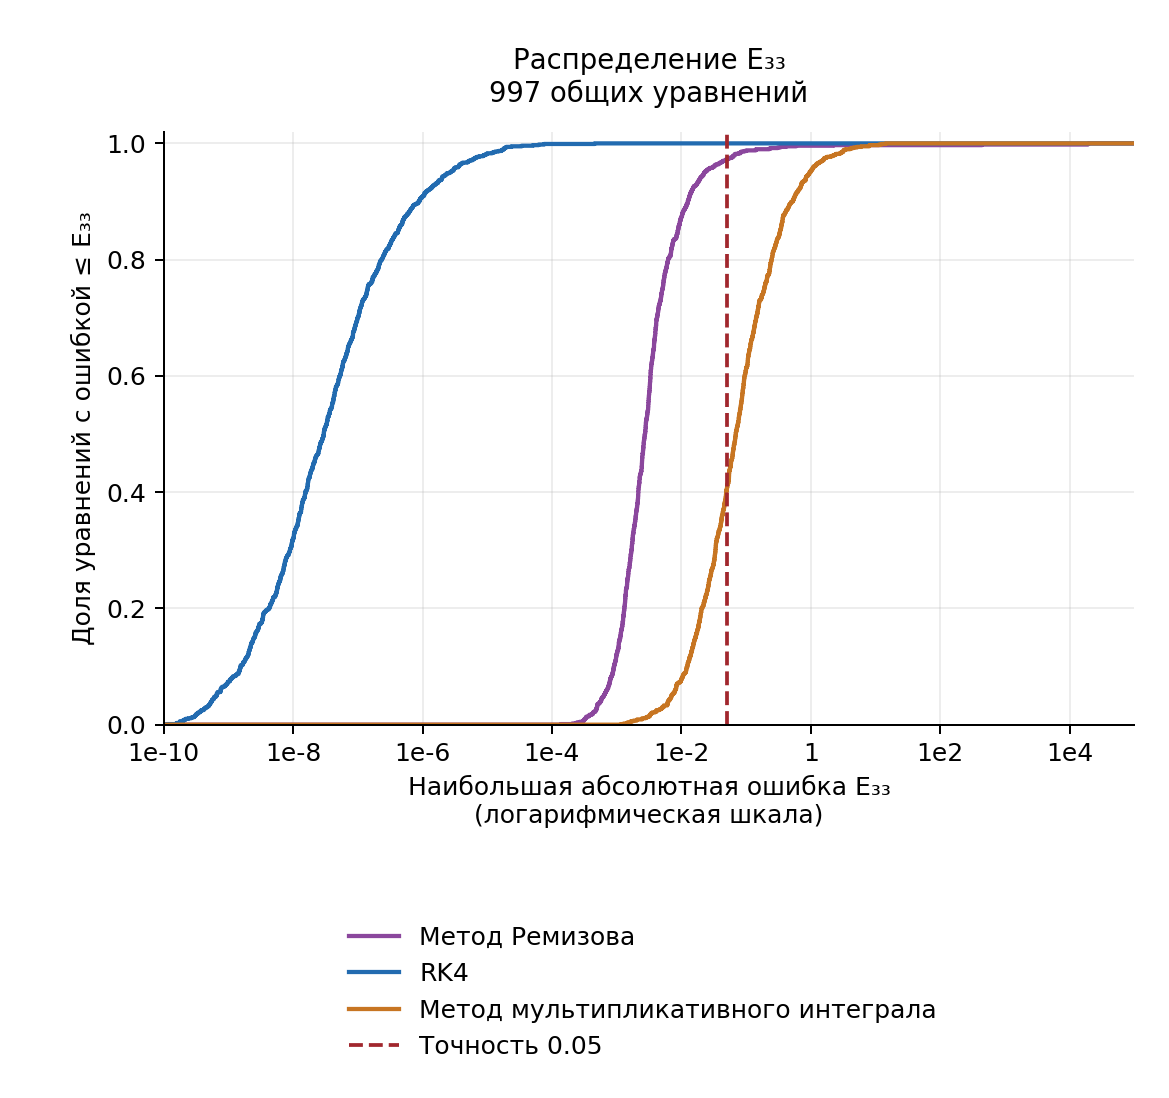
\includegraphics[width=\textwidth,height=0.8\textheight,keepaspectratio]{grid33_01_ecdf_common997.png}
\caption{Доля уравнений, на которых $E_{33}$ не больше заданного значения
(одни и те же 997 уравнений). Ось ошибок логарифмическая; пунктир ---
уровень $0.05$. Для Монте-Карло ошибки по 33 узлам нет.}
\label{fig:grid33-ecdf}
\end{figure}

\begin{figure}[!htbp]
\centering
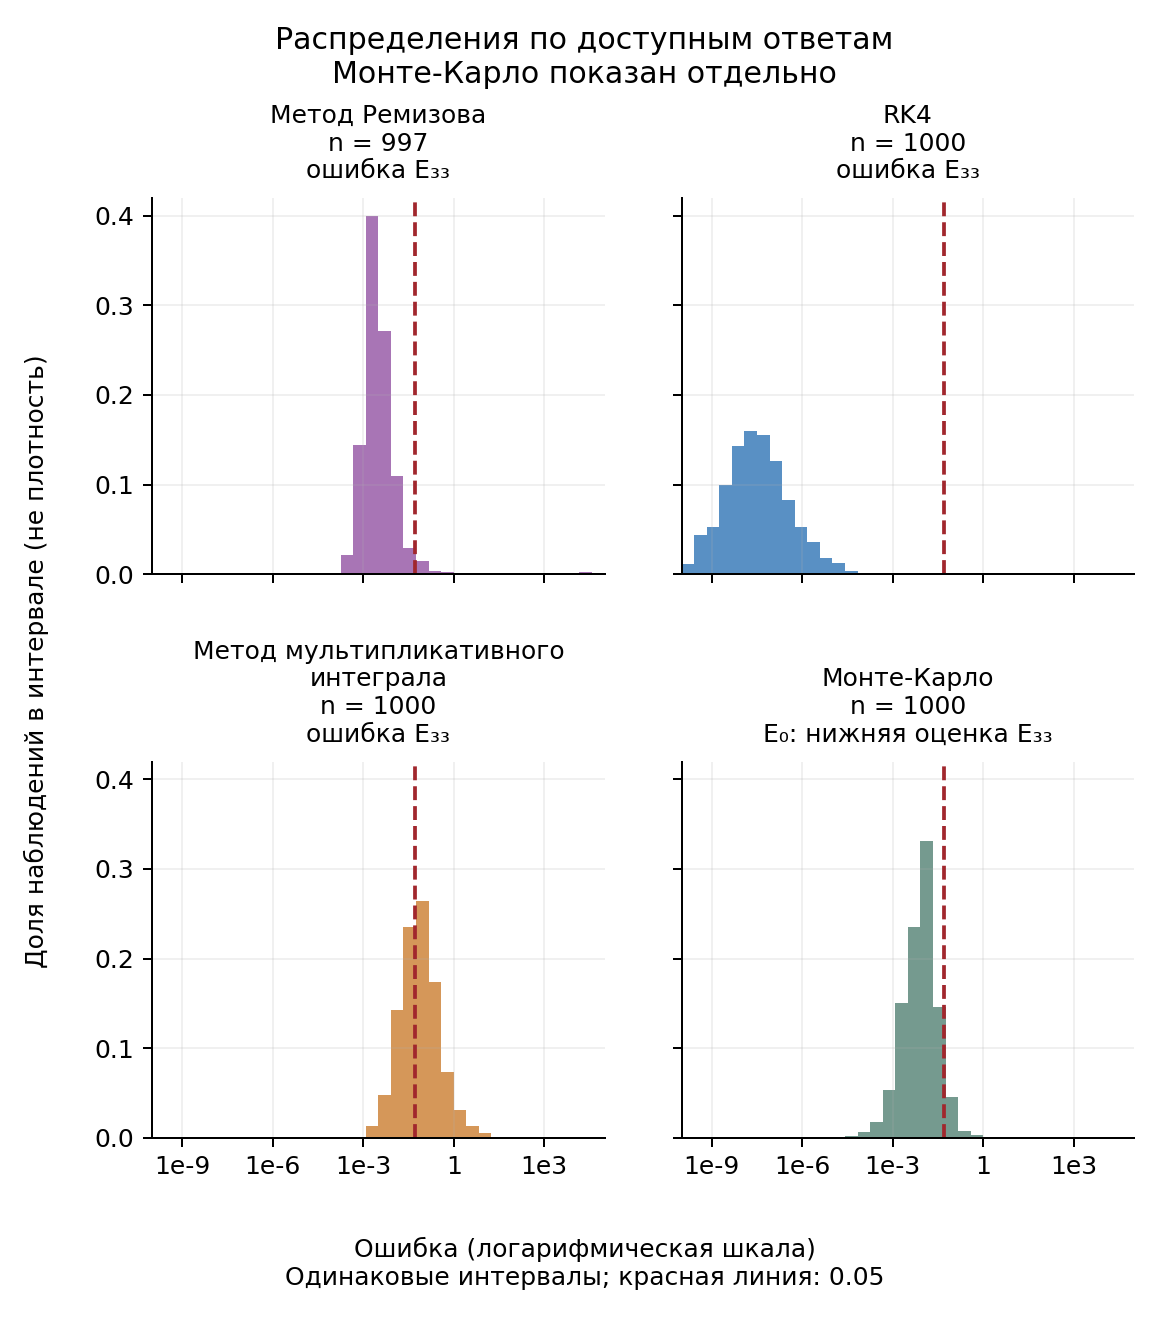
\includegraphics[width=\textwidth,height=0.8\textheight,keepaspectratio]{grid33_02_histograms_available.png}
\caption{Распределения ошибок по всем уравнениям, для которых есть ответ
метода; интервалы одинаковой ширины в логарифмической шкале. По
вертикали --- доля уравнений в интервале (не плотность). Для Монте-Карло
показана только ошибка в точке $x=0$ (оценка снизу). Пунктир ---
уровень $0.05$.}
\label{fig:grid33-hist}
\end{figure}

\begin{figure}[!htbp]
\centering
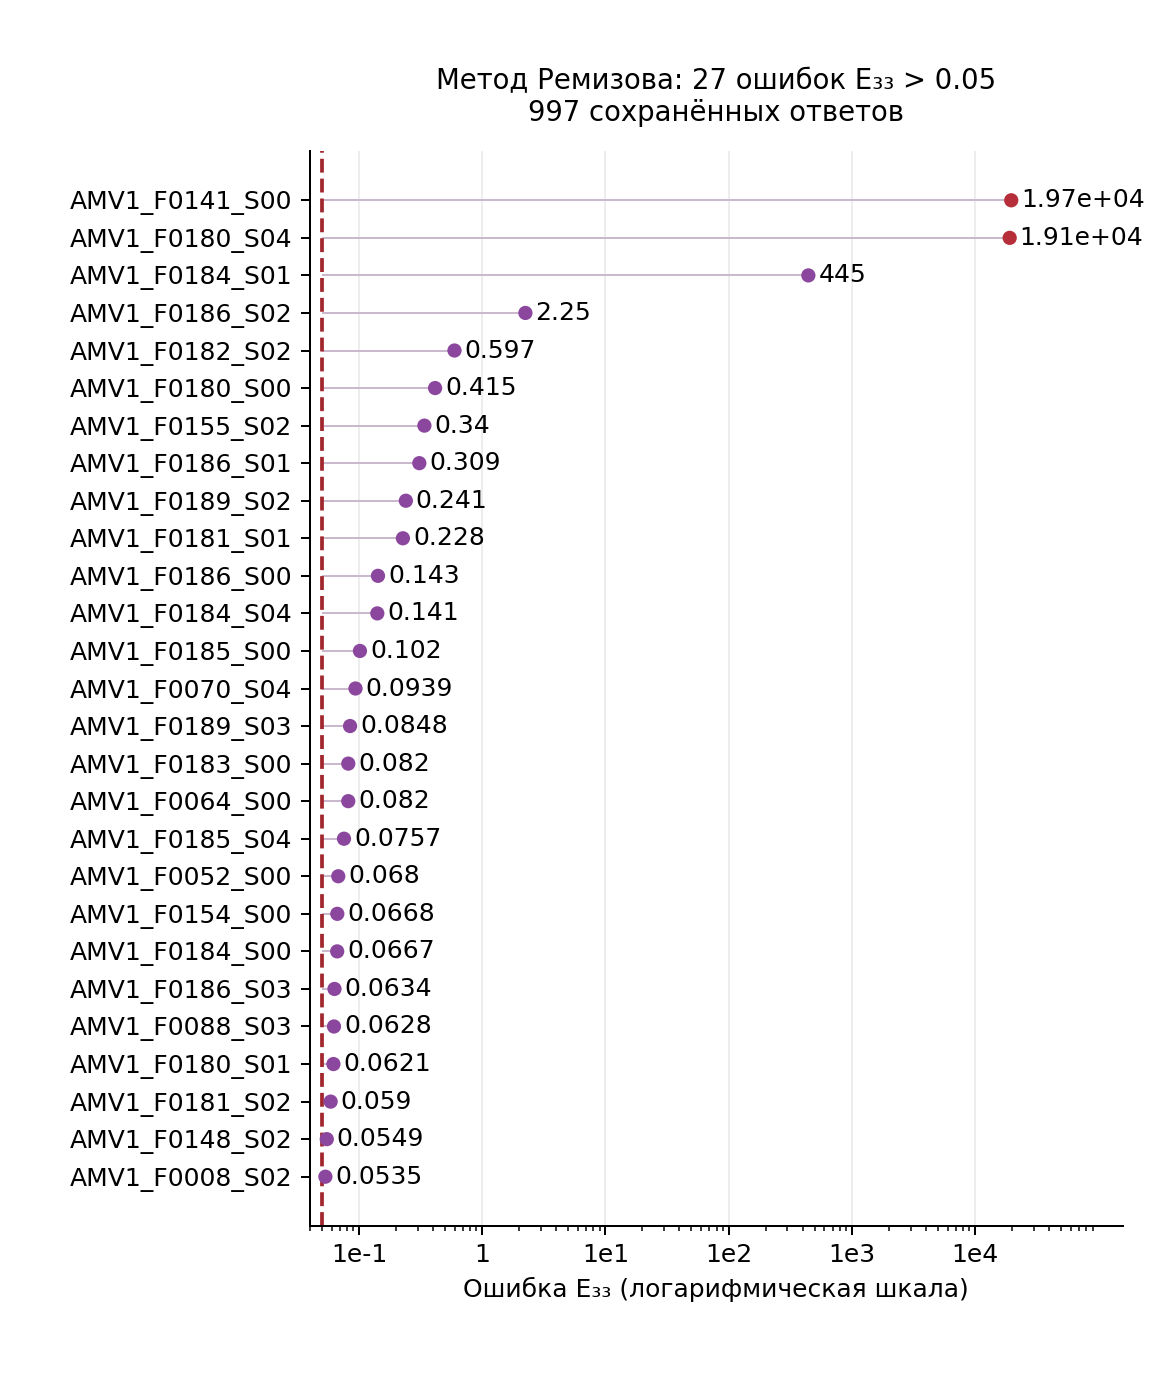
\includegraphics[width=\textwidth,height=0.8\textheight,keepaspectratio]{grid33_03_remizov_exceedances.png}
\caption{Все 27 уравнений, на которых $E_{\mathrm{R},33}>0.05$. Два самых
больших значения выделены цветом; из статистики они не удалялись.}
\label{fig:grid33-outliers}
\end{figure}

\begin{figure}[!htbp]
\centering
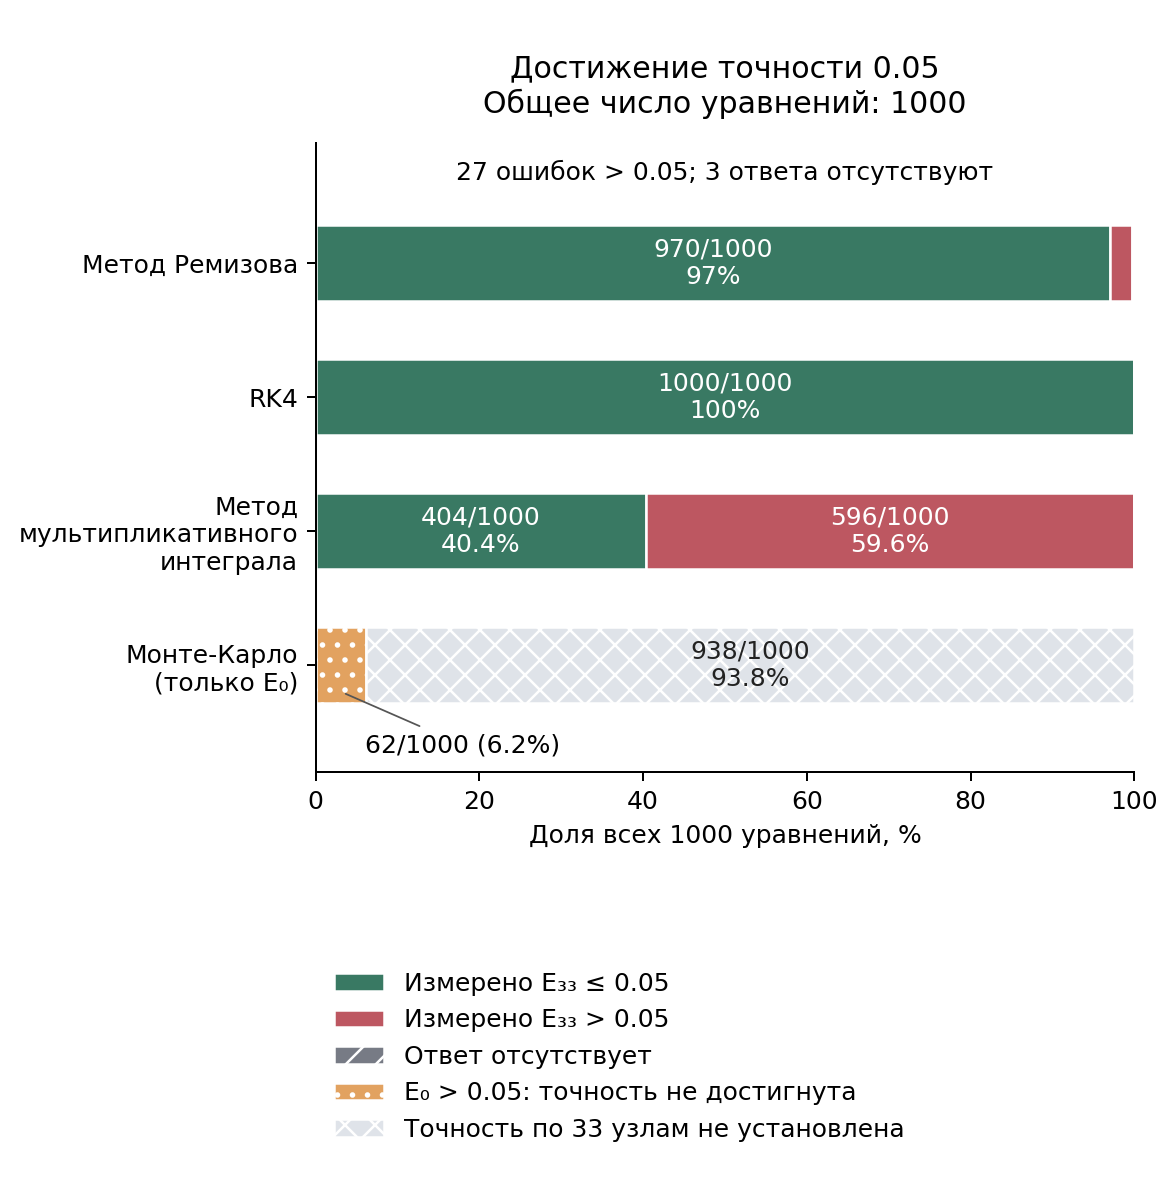
\includegraphics[width=\textwidth,height=0.8\textheight,keepaspectratio]{grid33_04_threshold_shares.png}
\caption{Доли от всех 1000 уравнений. Уравнения без ответа метода
Ремизова показаны отдельно от уравнений с ошибкой больше $0.05$.
Для Монте-Карло 62 случая недостижения точности следуют из оценки
снизу; на 938 уравнениях достижение точности неизвестно, и это
не 938 точных ответов.}
\label{fig:grid33-shares}
\end{figure}

\clearpage
\subsubsection{Время счёта при заданной точности: RK4 и мультипликативный интеграл}
\label{sec:costpilot}

То, что один метод точнее другого при фиксированных настройках, ещё
не означает, что выбор метода сокращает время счёта. Поэтому проведён
отдельный небольшой эксперимент: сравнивались только RK4
и мультипликативный интеграл при числе шагов $N=32,64,128,256$,
и требовалось $E_{m,33}\le0.01$. Модели выбора в этом эксперименте
не обучались.

\paragraph{Выборка и измерение времени\\}
Выбраны 60 уравнений из обучающей части, все из разных семейств: по три
уравнения из каждой из 20 комбинаций <<уровень сложности~$\times$~режим
коэффициентов>>. Уравнение-представитель семейства выбиралось
по фиксированному правилу, не зависящему от результатов. Уравнения
подбирались так, чтобы они как можно сильнее различались по входным
характеристикам: каждое следующее уравнение выбиралось с наибольшим
расстоянием до ближайшего из уже выбранных (по нормированным
характеристикам). Ошибки, времена и точные решения при выборе
не использовались; семейства из Test исключены. Такая выборка подобрана
по разнообразию, поэтому по ней нельзя оценивать, как часто что-либо
встречается в произвольном наборе уравнений.

Оба метода решали задачу Коши на $[-1,1]$ с одними и теми же
коэффициентами и точными начальными условиями $f(-1)$, $f'(-1)$.
При каждом $N$ узлы $G_{33}$ совпадают с узлами сетки метода
(с номерами $kN/32$, $k=0,\dots,32$), поэтому интерполяция не нужна.
Точность считается достигнутой и при равенстве $E_{m,33}=0.01$.

Каждое из $60\times8=480$ сочетаний <<уравнение~$\times$~вариант>>
запускалось на одном компьютере один раз пробно (без учёта времени)
и пять раз с измерением времени; порядок запусков перемешивался.
Время $t_i(m,N)$ --- медиана пяти измерений; в него входят вычисление
коэффициентов и сами шаги метода, но не входят загрузка данных,
вычисление ошибки и запись результатов. Проверить число внутренних
потоков вычислений и отсутствие замедления процессора из-за нагрева
не удалось, поэтому времена относятся только к этому компьютеру
и этой процедуре измерения.

\begin{table}[!htbp]
\centering
\caption{Точность и время восьми вариантов на 60 уравнениях. Время ---
среднее по уравнениям значение медианы пяти измерений.}
\label{tab:costpilot-configurations}
\small
\begin{tabular}{lrcrc}
\toprule
Метод & $N$ & $E_{m,33}\le0.01$ & Время, мс & $\max E_{m,33}$\\
\midrule
RK4 & 32  & 59/60 & 60.1  & $1.37\cdot10^{-2}$\\
RK4 & 64  & 60/60 & 120.0 & $2.75\cdot10^{-4}$\\
RK4 & 128 & 60/60 & 239.2 & $1.70\cdot10^{-5}$\\
RK4 & 256 & 60/60 & 479.0 & $1.06\cdot10^{-6}$\\
Мультипликативный интеграл & 32  & 0/60 & 15.7  & 15.92\\
Мультипликативный интеграл & 64  & 0/60 & 31.3  & 8.04\\
Мультипликативный интеграл & 128 & 4/60 & 62.7  & 4.04\\
Мультипликативный интеграл & 256 & 7/60 & 125.4 & 2.02\\
\bottomrule
\end{tabular}
\end{table}

\paragraph{Идеальный выбор и единые варианты\\}
Идеальный выбор для каждого уравнения берёт самый быстрый вариант среди
тех, что достигают точности $0.01$. Лучший единый вариант должен
достигать точности на всех 60 уравнениях и иметь наименьшую сумму
времён. Чтобы отделить выбор метода от выбора числа шагов, рассмотрен
также идеальный выбор только среди вариантов RK4. Все эти правила
используют уже известные ошибки и времена, поэтому показывают лишь
возможный выигрыш; время пробных расчётов для поиска подходящего $N$
в них не учтено.

\begin{table}[!htbp]
\centering
\caption{Время счёта при разных правилах выбора; во всех случаях
точность $0.01$ достигнута на всех 60 уравнениях.}
\label{tab:costpilot-selection}
\small
\begin{tabular}{>{\raggedright\arraybackslash}p{0.5\textwidth}rr}
\toprule
Правило выбора & Среднее, мс & Сумма, с\\
\midrule
Лучший единый вариант: RK4, $N=64$ & 120.0 & 7.20\\
Идеальный выбор из RK4 и мультипликативного интеграла & 62.0 & 3.72\\
Идеальный выбор только среди вариантов RK4 & 62.0 & 3.72\\
\bottomrule
\end{tabular}
\end{table}

Во всех 60 случаях идеальный выбор --- RK4; мультипликативный интеграл
не выбран ни разу. Для 59 уравнений достаточно $N=32$, для одного ---
$N=64$: у уравнения \texttt{AMV1\_F0186\_S00} при $N=32$
$E_{\mathrm{RK4},33}=0.0137$, при $N=64$ --- $2.10\cdot10^{-4}$.
Уравнений, на которых ни один вариант не достиг точности, нет; сбоев
расчёта тоже нет. Мультипликативный интеграл достигает точности хотя бы
при одном $N$ на семи уравнениях, но и там он медленнее подходящего
варианта RK4.

Идеальный выбор быстрее RK4 с $N=64$ в среднем на 49.2\%, а по сумме
времён --- на 48.3\%. Это разные величины:
\[
\frac1{60}\sum_{i=1}^{60}
\left(1-\frac{t_i^{\mathrm{ид}}}{t_i^{\mathrm{ед}}}\right),
\qquad
1-\frac{\sum_i t_i^{\mathrm{ид}}}{\sum_i t_i^{\mathrm{ед}}},
\]
где $t_i^{\mathrm{ид}}$ и $t_i^{\mathrm{ед}}$ --- время на $i$-м уравнении
при идеальном выборе и при едином варианте. В среднем экономится
57.9~мс на уравнение. Весь выигрыш даёт выбор числа шагов внутри RK4:
добавление мультипликативного интеграла не даёт дополнительного
выигрыша ($0\%$). Правило <<брать наименьшее $N$, при котором RK4
достигает точности>> совпало с идеальным выбором на всех 60 уравнениях.

До эксперимента были заранее заданы условия, при которых имело бы смысл
обучать модель выбора метода: каждый метод должен быть быстрее не менее
чем на 12 уравнениях из 60, причём не менее 12 раз --- уверенно; выигрыш
должен быть не меньше 10\% по обоим показателям относительно лучшего
единого варианта и относительно выбора только среди RK4; точность
должна достигаться на всех уравнениях, а измерения времени должны быть
стабильными не менее чем в 90\% случаев. Уверенная победа означает,
что медиана времени меньше хотя бы на 10\%, все пять измерений
быстрого варианта меньше всех пяти измерений медленного
($\max t_{\rm fast}<\min t_{\rm slow}$), а у обоих вариантов отношение
медианы абсолютных отклонений к медиане (MAD/median) не больше $0.20$.
Это практические условия, а не статистический тест. Условие на MAD
выполнено во всех 480 случаях; из 60 побед RK4 уверенными являются 56,
в четырёх запас не подтверждён, но и это не победы мультипликативного
интеграла.

\textbf{Итог: обучать модель выбора между RK4 и мультипликативным
интегралом в такой постановке нецелесообразно.} Самый быстрый метод
не меняется от уравнения к уравнению, мультипликативный интеграл
не выигрывает ни разу, и дополнительного выигрыша по сравнению с выбором
$N$ только у RK4 нет. Отдельно не проверялось, полезно ли заранее
предсказывать редкие случаи, когда RK4 нужно больше шагов. Эксперимент
не доказывает ни возможности обучить модель выбора, ни переносимости
времён на другие компьютеры, ни порядка сходимости, ни превосходства
RK4 в общем случае. Все числа перепроверены по сохранённым данным
без новых расчётов.

\clearpage
\subsubsection{Продолжение за край окна в методе Ремизова}
\label{sec:boundarydev}

Ранее на двух уравнениях с очень большой ошибкой было замечено, что
ошибка сильно уменьшается, если за краем окна продолжать функцию нулём,
а не с плавным затуханием. Чтобы проверить, насколько это общее
явление, проведено одно отдельное исследование. В нём проверяется
конкретная численная реализация на конечном окне; формула метода
и основной вариант расчёта (с плавным затуханием) не меняются.
Обозначим через $E^{(1)}$ ошибку $E_{\mathrm{R},33}$ при исходном
продолжении (плавное затухание), а через $E^{(0)}$ --- при продолжении
нулём.

\paragraph{Выборка и что менялось\\}
Взяты все 22 уравнения вне Test, на которых $E^{(1)}>0.05$,
и 30 заранее выбранных контрольных уравнений с $E^{(1)}\le0.05$.
Проблемные уравнения относятся к 14 семействам; контрольные взяты
из 30 других, попарно различных семейств, с равномерным охватом
20 комбинаций <<уровень сложности~$\times$~режим>>. Семейства из Test
исключены, ответы с продолжением нулём при отборе не использовались.
Три уравнения без ответа метода Ремизова в выборку не входят.
Уравнение \texttt{AMV1\_F0180\_S04} относится к Test и поэтому сюда
не включено; в прежнем расчёте его ошибка при продолжении нулём
уменьшилась с 19134.4 до 0.0705, то есть осталась больше $0.05$.

Для всех 52 уравнений использованы уже сохранённые ответы с плавным
затуханием; ответы с продолжением нулём для двух уравнений были
сохранены раньше, для остальных 50 вычислены заново. Менялся только
способ продолжения за край окна. Остальное то же: $n=128$, 513 узлов
по $t$ с размещением $t_j=T(j/512)^2$, $\Delta x=0.0125$, окно $[-13,13]$
(2081 узел), $\varepsilon_T=10^{-8}$; значение $T$ для каждого уравнения
совпадает. Совпадение коэффициентов, точных решений, сеток, весов
квадратуры и узлов $G_{33}$ проверено. Другие способы продолжения,
а также Монте-Карло и модели выбора здесь не рассматривались.

Требуемая точность --- $0.05$. Ошибку $E_{\mathrm{R},33}>1$ будем
называть очень большой; это только название, а не утверждение, что
метод неприменим. Для разности $\Delta E=E^{(0)}-E^{(1)}$ заранее задан
порог
\[
\delta_i=10^{-10}\max\{1,E_i^{(1)}\}.
\]
Ошибка считается уменьшившейся, если $\Delta E<-\delta_i$,
не изменившейся, если $|\Delta E|\le\delta_i$, и увеличившейся, если
$\Delta E>\delta_i$. Порог $\delta_i$ нужен только для сравнения чисел
и не является ни оценкой полной ошибки, ни границей практической
заметности.

\begin{table}[!htbp]
\centering
\caption{Результат замены плавного затухания на продолжение нулём.
Уменьшение, неизменность и увеличение ошибки определены с порогом
$\delta_i$. В столбцах <<до/после>> указано число уравнений при исходном
продолжении и при продолжении нулём.}
\label{tab:boundarydev-groups}
\resizebox{\textwidth}{!}{%
\begin{tabular}{lrrrrrr}
\toprule
Группа & Уравнений & \parbox{23mm}{\centering $E_{33}\le0.05$, до/после} & Уменьшилась & Не изменилась
 & Увеличилась & \parbox{20mm}{\centering $E_{33}>1$, до/после}\\
\midrule
Проблемные & 22 & 0/1 & 9 & 10 & 3 & 3/0\\
Контрольные & 30 & 30/30 & 2 & 28 & 0 & 0/0\\
Все & 52 & 30/31 & 11 & 38 & 3 & 3/0\\
\bottomrule
\end{tabular}}
\end{table}

\paragraph{Что изменилось\\}
Все три очень большие ошибки стали меньше единицы
(таблица~\ref{tab:boundarydev-extremes}). Значит, для этих уравнений
большие ошибки действительно связаны со способом продолжения за край
окна: остальные параметры не менялись. Однако точности $0.05$ достигло
только одно из 22 проблемных уравнений; на 21 ошибка осталась больше
$0.05$. Наибольшая ошибка по 52 уравнениям уменьшилась с 19704.5
до 0.597. На всех 30 контрольных уравнениях точность сохранилась;
новых ошибок больше единицы и сбоев расчёта нет.

\begin{table}[!htbp]
\centering
\caption{Три очень большие ошибки ($E_{33}>1$) до и после замены.
Приведены итоговые ошибки в узлах $G_{33}$, а не промежуточные значения.}
\label{tab:boundarydev-extremes}
\small
\begin{tabular}{lrrc}
\toprule
Уравнение & $E^{(1)}$ & $E^{(0)}$ & Точность $0.05$ после\\
\midrule
\texttt{AMV1\_F0141\_S00} & 19704.5 & 0.0187 & да\\
\texttt{AMV1\_F0184\_S01} & 444.6 & 0.0536 & нет\\
\texttt{AMV1\_F0186\_S02} & 2.246 & 0.254 & нет\\
\bottomrule
\end{tabular}
\end{table}

Если не учитывать порог $\delta_i$, ошибка выросла на 19 уравнениях,
но только в трёх случаях рост больше $\delta_i$
(таблица~\ref{tab:boundarydev-regressions}). Все три уравнения и до
замены имели ошибку больше $0.05$, так что точность нигде не потеряна.
Рост порядка $10^{-9}$ практически незаметен.

\begin{table}[!htbp]
\centering
\caption{Три случая, где ошибка выросла больше чем на $\delta_i$.
Относительный рост дан как доля, а не в процентах.}
\label{tab:boundarydev-regressions}
\small
\begin{tabular}{lcc}
\toprule
Уравнение & $\Delta E$ & $\Delta E/E^{(1)}$\\
\midrule
\texttt{AMV1\_F0186\_S01} & $6.10\cdot10^{-10}$ & $1.97\cdot10^{-9}$\\
\texttt{AMV1\_F0189\_S02} & $1.31\cdot10^{-9}$ & $5.46\cdot10^{-9}$\\
\texttt{AMV1\_F0189\_S03} & $6.15\cdot10^{-10}$ & $7.25\cdot10^{-9}$\\
\bottomrule
\end{tabular}
\end{table}

\paragraph{Ограничения численной схемы по $x$\\}
При продолжении нулём внутри окна используется тот же кубический
сплайн, а в точках строго за окном значение полагается равным нулю.
Значение в крайнем узле окна при этом не обнуляется. Если оно не равно
нулю, продолжение разрывно и не лежит в пространствах непрерывных
ограниченных функций $C_b$ или $UC_b$, которые нужны в теоретическом
обосновании метода. Это и не решение краевой задачи с нулевыми
граничными условиями: значения в крайних узлах не обнуляются. Даже если
значения на концах равны нулю, продолжение может быть негладким.
Например, кубический сплайн по узлам $x=(0,1,2,3)$ со значениями
$(0,1,1,0)$ равен $p(x)=3x/2-x^2/2$; его производные на концах равны
$3/2$ и $-3/2$, а у нулевого продолжения производная равна нулю.

Проверки показывают также, что численная операция <<построить
кубический сплайн по значениям в узлах и вычислить сдвиги>> может
не сохранять неотрицательность и может увеличивать максимум модуля
по узлам. При $x=(0,1,2,3)$, $a=1/4$, $b=4$, $c=0$, $\tau=1/16$
и продолжении нулём одно применение $S(\tau)$ к данным $u=(0,1,1,0)$
(максимум модуля равен 1) даёт в узле $x=1$ значение $67/64>1$, а для
неотрицательных данных $u=(1,0,0,0)$ --- значение $-1/64$ в том же
узле. Это примеры для численной операции над значениями в узлах,
а не для точного оператора $S$ на непрерывных функциях: сам сплайн
может выходить за пределы диапазона значений в узлах. То, что веса
$1/4,1/4,1/2$ неотрицательны и в сумме дают 1, ещё не даёт оценки
нормы численного оператора.

Правая часть $g$ равна нулю вне некоторого отрезка внутри окна, но
при повторных сдвигах ненулевые значения доходят до краёв окна.
Поэтому то, что $g$ равна нулю у краёв окна, не исключает влияния
границы окна. Наибольшее по модулю промежуточное значение у края окна,
сохранённое при расчёте, описывает именно эти промежуточные значения
и не равно итоговой ошибке $E_{\mathrm{R},33}$. Формула $S$
и коэффициенты (вместе с их границами) не менялись; однако
устойчивость численной схемы по $x$, ошибка от конечного окна
и выполнение всех условий теоремы для этой конечномерной реализации
не доказаны. Измельчение $\Delta x$, расширение окна, изменение $T$,
квадратуры и $n$ в этом сравнении не проводились, поэтому неизвестно,
какая часть оставшейся ошибки приходится на каждый источник.

До получения новых ответов были заданы условия успеха: все расчёты
выполнены без сбоев; ни одна ошибка не увеличилась больше чем
на $\delta_i$; точность $0.05$ нигде не потеряна; нет новых ошибок
больше единицы; все прежние ошибки больше единицы устранены; число
уравнений с достигнутой точностью выросло; хотя бы одна ошибка
уменьшилась больше чем на $\delta_i$. Не выполнено только условие
<<ни одна ошибка не увеличилась>>. \textbf{Формальный итог: по этому
заранее заданному правилу продолжение нулём не принимается как новый
вариант расчёта.} Условия после получения результатов не менялись.
Итог зависит от строгости порога $\delta_i$ и не означает, что
продолжение нулём практически хуже: сильное уменьшение трёх очень
больших ошибок остаётся установленным результатом. В то же время
продолжение нулём устраняет не все большие ошибки и не делает
численную схему по $x$ теоретически обоснованной. Основной вариант
расчёта и основные таблицы не менялись. Все числа этого раздела
перепроверены по сохранённым данным без повторного решения уравнений.


\subsubsection{Выбор из трёх методов}\label{sec:ml3-res}
Если не рассматривать RK4, лучшими оказываются разные методы:
на 997 уравнениях метод Ремизова точнее двух других на 826, Монте-Карло ---
на 106, мультипликативный интеграл --- на 65 (рис.~\ref{fig:ml3-wins},
таблица~\ref{tab:ml3-split}). Результаты модели на тестовой выборке
приведены в таблице~\ref{tab:ml3-test}.

\begin{figure}[!htbp]
\centering
\includegraphics[width=0.8\textwidth]{01_winners.png}
\caption{Число уравнений, на которых каждый из трёх методов даёт
наименьшую ошибку в точке $x=0$ (997 уравнений). R128 --- метод Ремизова
при $n=128$, MC mean4 --- среднее четырёх расчётов Монте-Карло,
PI --- метод мультипликативного интеграла.}
\label{fig:ml3-wins}
\end{figure}

\begin{table}[!htbp]
\centering
\caption{Модель выбора из трёх методов и постоянный выбор одного метода
на тестовой выборке (150 уравнений).}
\label{tab:ml3-test}
\resizebox{\textwidth}{!}{%
\begin{tabular}{lcccc}
\toprule
Правило выбора & Accuracy & macro-F1 & $E\le0.05$ & средняя $E$\\
\midrule
модель & 88.67\% & 0.314 & 147/150 & 1.65885\\
всегда метод Ремизова & 90.67\% & 0.317 & 147/150 & 1.65896\\
всегда Монте-Карло & 4.67\% & 0.030 & 141/150 & 0.01728\\
всегда мультипликативный интеграл & 4.67\% & 0.030 & 110/150 & 0.05416\\
\bottomrule
\end{tabular}}
\end{table}

Модель верно определила лучший метод на 133 из 150 тестовых уравнений
(88.67\%), а выбранный ею метод достиг точности $0.05$ на 147 уравнениях
(98\%). Постоянный выбор метода Ремизова верен на 136 уравнениях
(90.67\%) и тоже достигает точности на 147. Модель выбрала метод
Ремизова 146 раз, Монте-Карло --- 4 раза, мультипликативный интеграл
не выбрала ни разу.

Матрица ошибок модели (строки --- метод, который на самом деле точнее,
столбцы --- выбор модели; порядок: метод Ремизова, Монте-Карло,
мультипликативный интеграл) имеет вид
\[
\begin{pmatrix}
133&3&0\\
7&0&0\\
6&1&0
\end{pmatrix}
\]
(рис.~\ref{fig:ml3-conf}). Все четыре выбора Монте-Карло ошибочны:
в трёх случаях точнее был метод Ремизова, в одном --- мультипликативный
интеграл. Ни одно из 7 уравнений, где точнее Монте-Карло, и ни одно
из 7, где точнее мультипликативный интеграл, модель не нашла. Поэтому
для этих двух методов $F_1=0$, и macro-F1 у модели и у постоянного
выбора метода Ремизова почти одинаков и мал (рис.~\ref{fig:ml3-acc}).

\begin{figure}[!htbp]
\centering
\begin{minipage}[t]{0.49\textwidth}
\centering
\includegraphics[width=\linewidth]{02_accuracy.png}
\end{minipage}\hfill
\begin{minipage}[t]{0.49\textwidth}
\centering
\includegraphics[width=\linewidth]{03_macro_f1.png}
\end{minipage}
\caption{Доля верных выборов (слева) и macro-F1 (справа) на тестовой
выборке для модели и для постоянного выбора метода Ремизова
(на рисунке --- <<Всегда R128>>).}
\label{fig:ml3-acc}
\end{figure}

\begin{figure}[!htbp]
\centering
\includegraphics[width=0.6\textwidth]{05_confusion_matrix.png}
\caption{Матрица ошибок модели выбора из трёх методов на тестовой
выборке: по строкам --- метод, который на самом деле точнее,
по столбцам --- метод, выбранный моделью. R128 --- метод Ремизова,
MC mean4 --- Монте-Карло, PI --- мультипликативный интеграл.}
\label{fig:ml3-conf}
\end{figure}

Средние ошибки модели и постоянного выбора метода Ремизова почти
совпадают (рис.~\ref{fig:ml3-mean}). Значение $1.659$ для постоянного
выбора метода Ремизова то же, что в таблице~\ref{tab:ml-rules}, и, как
показано в разделе~\ref{sec:ml-res2}, почти целиком определяется одним
уравнением \texttt{AMV1\_F0180\_S04}, где $E_{\mathrm{R}}=248.3$. Средняя
ошибка модели почти так же велика: по сохранённым ответам модели
на этом уравнении она тоже выбрала метод Ремизова.

\begin{figure}[!htbp]
\centering
\includegraphics[width=0.85\textwidth]{04_mean_error.png}
\caption{Средняя ошибка выбранного метода в точке $x=0$ на тестовой
выборке для модели и для постоянного выбора одного метода. R128 ---
метод Ремизова, MC mean4 --- Монте-Карло, PI --- мультипликативный
интеграл.}
\label{fig:ml3-mean}
\end{figure}

На рис.~\ref{fig:ml3-imp} показаны пять признаков с наибольшей
важностью. Важность --- вычисляемая CatBoost оценка того, насколько
признак в среднем меняет ответы модели; сумма важностей всех 258
признаков равна 100\%.
Наиболее важны среднеквадратичное значение $b$ (10.36\%; приложение,
П.2, величина 5), значение $b$ в узле $x\approx0.545$ (5.15\%; П.1),
число $\lambda$ (4.85\%; П.5), полная вариация коэффициента $a$
(4.62\%; П.2, величина 8) и величина $\sqrt{2A_+T}$ (4.27\%; П.6,
величина 7). Вместе на них приходится около 29\% суммарной важности.
Важность показывает, какими признаками модель пользуется больше всего,
но не объясняет, почему один метод точнее другого.

\begin{figure}[!htbp]
\centering
\includegraphics[width=0.85\textwidth]{06_top5_features.png}
\caption{Пять признаков с наибольшей важностью в модели выбора из трёх
методов. <<Значение b (b\_sample\_24)>> --- значение $b$ в узле
$x\approx0.545$; <<Изменчивость a>> --- полная вариация $a$ (приложение,
П.2, величина 8); <<Диффузионная длина>> --- величина $\sqrt{2A_+T}$.}
\label{fig:ml3-imp}
\end{figure}

Таким образом, построен и проверен полный процесс автоматического выбора
одного из трёх методов по признакам уравнения, но на тестовой выборке
модель не лучше постоянного выбора метода Ремизова: доля верных выборов
у неё на 2 процентных пункта меньше, а число уравнений с достигнутой
точностью и средняя ошибка практически те же. Результат относится
к фиксированным настройкам методов и к ошибке в точке $x=0$; тестовая
выборка ранее использовалась в других расчётах проекта, поэтому оценка
не является полностью независимой.

\section{Заключение}
\subsection{Краткие выводы по полученным результатам}
\begin{enumerate}
\item Построен набор из 1000 уравнений с известными точными решениями,
в котором коэффициент $a$ положителен и $\lambda>\sup_x|c(x)|$
по построению, и получены ошибки четырёх численных методов в точке
$x=0$.
\item Метод Ремизова точнее Монте-Карло на 881 уравнении из 997
и достигает точности $0.05$ на 982 из них, но изредка его ошибка
на несколько порядков больше (до 842).
\item Выбранная по Validation модель выбора из двух методов
(253 признака) имеет на Test accuracy 91.33\% и macro-F1 0.544, а выбранный
ею метод достигает точности $0.05$ на 146 уравнениях из 150; её средняя
ошибка не меньше, чем при постоянном выборе метода Ремизова. Модель
с 258 признаками находит 6 из 9 тестовых уравнений, где точнее
Монте-Карло, но делает 14 ошибочных выборов и 3 пропуска; два ошибочных
выбора приводят к потере точности $0.05$. Её выигрыш в средней ошибке
определяется одним уравнением, поэтому устойчивого преимущества перед
постоянным выбором метода Ремизова нет. Выводы ограничены повторным
использованием тестовой выборки и малым числом уравнений, где точнее
Монте-Карло.
\item Выбор более точного метода и достижение точности $0.05$ ---
разные свойства: верно выбранный метод может не достигать точности.
\item При выбранных настройках RK4 точнее остальных методов в точке
$x=0$ на всех 997 уравнениях и достигает точности $0.05$ на всех 1000,
поэтому выбор из четырёх методов на этом наборе тривиален. Это результат
для данного набора и данных настроек, а не доказательство превосходства
RK4 в общем случае.
\item По наибольшей ошибке в 33 узлах RK4 тоже точнее остальных
методов на всех 997 общих уравнениях. Для Монте-Карло использована
только оценка снизу через ошибку в точке $x=0$; значений во всех узлах
для него нет. Точность $0.05$ по 33 узлам достигается у метода Ремизова
на 970 из 997 уравнений, у RK4 --- на 1000 из 1000, у мультипликативного
интеграла --- на 404 из 1000. Оценки наибольшей ошибки на всём отрезке
нет.
\item Модель выбора из трёх методов --- Ремизова, Монте-Карло и метода
мультипликативного интеграла --- верно определяет лучший метод
на 88.67\% тестовых уравнений, а выбранный ею метод достигает точности $0.05$
на 98\% из них. Однако постоянный выбор метода Ремизова даёт 90.67\%
и те же 98\%: модель почти всегда выбирает метод Ремизова (146 раз
из 150) и не находит ни одного уравнения, где точнее другой метод.

\item На 60 уравнениях вне Test при требовании $E_{33}\le0.01$ идеальный
выбор по времени счёта всегда даёт RK4 (59 раз $N=32$, один раз $N=64$).
Он быстрее единого варианта RK4 с $N=64$ в среднем на 49.2\% (по сумме
времён --- на 48.3\%), но по сравнению с выбором $N$ только у RK4
выигрыш равен нулю. Поэтому обучать модель выбора между RK4
и мультипликативным интегралом в такой постановке нецелесообразно.
\item При продолжении нулём за край окна все три ошибки метода Ремизова
$E_{33}>1$ стали меньше единицы, на контрольных уравнениях точность
сохранилась (30 из 30), а среди проблемных уравнений точность достигнута
на одном из 22 (раньше ни на одном). Заранее заданное строгое условие
<<ни одна ошибка не увеличилась>> не выполнено из-за трёх увеличений
порядка $10^{-9}$, что практически незаметно. На 21 уравнении ошибка
осталась больше $0.05$, а теоретические ограничения численной схемы
по $x$ сохраняются. Основной вариант расчёта не заменялся.
\end{enumerate}

\subsection{Оценка полноты решения поставленных задач и планируемое развитие}
Все поставленные задачи выполнены: построены набор уравнений
и признаки, получены ошибки четырёх методов в точке $x=0$, исследованы
модели выбора из двух методов, разобраны неверные выборы модели с 258
признаками и проверена модель выбора из трёх методов. По сохранённым
данным получены ошибки методов Ремизова, RK4 и мультипликативного
интеграла в 33 узлах и с помощью оценки снизу для Монте-Карло показано,
что RK4 остаётся самым точным. Отдельно проведены эксперимент по времени
счёта и проверка продолжения за край окна (разделы~\ref{sec:costpilot}
и~\ref{sec:boundarydev}). При подготовке этого текста новых расчётов
и обучений моделей не проводилось; использованы только сохранённые
результаты.

Открытыми остаются следующие вопросы:
\begin{enumerate}
\item Ошибка Монте-Карло во всех 33 узлах, её случайный разброс и ошибка
от конечного шага по времени; обучение моделей выбора по ошибке
в 33 узлах.
\item Ошибка между узлами сетки и расчёты с последовательным
измельчением шага; время, нужное для достижения точности, за пределами
проведённого эксперимента, с учётом времени пробных расчётов для выбора
числа шагов.
\item Устойчивость численной схемы метода Ремизова по $x$, контроль
влияния границы окна и разделение оставшейся ошибки после замены
продолжения; причины трёх прерванных расчётов.
\item Проверка моделей выбора на новых семействах уравнений и на новой
тестовой выборке; сравнение методов при одинаковых для всех методов
начальных данных.
\end{enumerate}
Эти вопросы не отменяют полученных результатов, но ограничивают
их толкование. Из текущих данных не следует, что более сложные модели
или новые уравнения без конкретной проверяемой гипотезы улучшат
результат.

\clearpage
\renewcommand{\refname}{Список использованных источников}
\phantomsection
\addcontentsline{toc}{section}{Список использованных источников}
\begin{thebibliography}{9}
\raggedright
\bibitem{repo2488} Timofeev, M. Yu.. ode-generator-remizov: генератор уравнений, решатели и эксперименты по выбору метода. GitHub. 2026. URL: \url{https://github.com/MikTi05/ode-generator-remizov}.

\end{thebibliography}

\clearpage
\section*{Приложение. Признаки модели выбора метода}
\phantomsection
\addcontentsline{toc}{section}{Приложение. Признаки модели выбора метода}

Признаки вычисляются по функциям $v\in\{a,b,c,g\}$ из
уравнения~\eqref{eq:ode} на сетке $x_i=-1+2i/255$, $i=0,\dots,255$;
$v_i=v(x_i)$. Всего признаков
\[
258=128+56+6+48+5+10+5.
\]

\subsection*{П.1. Значения функций (128 признаков)}
Для каждой функции $v\in\{a,b,c,g\}$ берутся 32 значения
\[
v\bigl(x_{j_k}\bigr),\qquad j_k=\lfloor 255k/31\rfloor,\quad k=0,\dots,31,
\]
то есть значения в почти равноотстоящих узлах от $x=-1$ до $x=1$.
Значения берутся в узлах сетки, без интерполяции.

\subsection*{П.2. Статистики функций (56 признаков)}
Для каждой функции $v\in\{a,b,c,g\}$ вычисляются 14 величин из
таблицы~\ref{tab:app-stats}. Обозначения:
\begin{gather*}
\bar v=\frac1{256}\sum_{i=0}^{255}v_i,\qquad
d^{(1)}_i=\frac{v_{i+1}-v_i}{x_{i+1}-x_i},\quad i=0,\dots,254,\\
d^{(2)}_i=\frac{d^{(1)}_{i+1}-d^{(1)}_i}{m_{i+1}-m_i},\quad i=0,\dots,253,
\end{gather*}
где $m_i=(x_i+x_{i+1})/2$ --- середины отрезков сетки;
$d^{(1)}$ и $d^{(2)}$ --- разностные оценки первой и второй производных.
Через $\hat v_k$ обозначено дискретное преобразование Фурье
последовательности $v_i-\bar v$, $P_k=|\hat v_k|^2$, $k=0,\dots,128$.

\begin{table}[!htbp]
\centering
\caption{Статистики, вычисляемые для каждой из функций $a,b,c,g$.}
\label{tab:app-stats}
\renewcommand{\arraystretch}{1.25}
\begin{tabular}{r>{\raggedright\arraybackslash}p{0.4\textwidth}l}
\toprule
№ & Величина & Формула\\
\midrule
1 & максимум & $\max_i v_i$\\
2 & минимум & $\min_i v_i$\\
3 & среднее & $\bar v$\\
4 & стандартное отклонение & $\Bigl(\frac1{256}\sum_i(v_i-\bar v)^2\Bigr)^{1/2}$\\
5 & среднеквадратичное значение & $\Bigl(\frac1{256}\sum_i v_i^2\Bigr)^{1/2}$\\
6 & максимум модуля & $\max_i|v_i|$\\
7 & медиана & медиана чисел $v_0,\dots,v_{255}$\\
8 & полная вариация & $\sum_{i=0}^{254}|v_{i+1}-v_i|$\\
9 & среднеквадратичная первая производная & $\Bigl(\frac1{255}\sum_i\bigl(d^{(1)}_i\bigr)^2\Bigr)^{1/2}$\\
10 & максимум модуля первой производной & $\max_i\bigl|d^{(1)}_i\bigr|$\\
11 & среднеквадратичная вторая производная & $\Bigl(\frac1{254}\sum_i\bigl(d^{(2)}_i\bigr)^2\Bigr)^{1/2}$\\
12 & доля отрицательных значений & $\frac1{256}\,\#\{i:\ v_i<0\}$\\
13 & число смен знака & $\#\{i:\ v_iv_{i+1}<0\}$\\
14 & доля высоких частот & $\sum_{k\ge8}P_k\big/\sum_kP_k$\\
\bottomrule
\end{tabular}
\end{table}
Если $\sum_kP_k=0$ (функция постоянна), величина 14 полагается равной нулю.

\subsection*{П.3. Корреляции (6 признаков)}
Для каждой пары функций $(a,b)$, $(a,c)$, $(a,g)$, $(b,c)$, $(b,g)$,
$(c,g)$ вычисляется коэффициент корреляции значений на сетке
\[
\rho(v,w)=\frac{\sum_i(v_i-\bar v)(w_i-\bar w)}
{\sqrt{\sum_i(v_i-\bar v)^2}\,\sqrt{\sum_i(w_i-\bar w)^2}};
\]
если одна из функций постоянна, полагается $\rho=0$.

\subsection*{П.4. Характеристики формул коэффициентов (48 признаков)}
Формулы $T_a,T_b,T_c$ из~\eqref{eq:ml-coef} записываются в виде дерева
операций (до преобразования $\tanh$). Для каждой из трёх формул
вычисляются 16 величин: общее число узлов дерева, глубина дерева
(корень имеет глубину 1) и число узлов каждого из 14 видов
из таблицы~\ref{tab:app-ops}. Числовые параметры $\alpha,\beta,\omega,
\varphi,\mu$ в признаки не входят. Формула точного решения не используется.

\begin{table}[!htbp]
\centering
\caption{Виды узлов в формулах коэффициентов.}
\label{tab:app-ops}
\renewcommand{\arraystretch}{1.3}
\begin{tabular}{>{\raggedright\arraybackslash}p{0.32\textwidth}l}
\toprule
Тип узла & Вид\\
\midrule
функции от $x$ (листья) & константа;\ $\sin(\omega x+\varphi)$;\ $\cos(\omega x+\varphi)$;\\
 & $\tanh(\omega x+\varphi)$;\ $e^{-\alpha(x-\mu)^2}$;\\
 & $\dfrac{1}{1+\alpha(x-\mu)^2}$;\ $\dfrac{x-\mu}{\sqrt{1+(x-\mu)^2}}$\\
\midrule
функции одного аргумента $u$ & $\sin u$;\ $\cos u$;\ $\tanh u$;\ $e^{-u^2}$;\ $\dfrac{u}{1+u^2}$\\
\midrule
функции двух аргументов $u,w$ & $\alpha u+\beta w$;\ $u\cdot w$\\
\bottomrule
\end{tabular}
\end{table}

В функциях $e^{-\alpha(x-\mu)^2}$ и $1/(1+\alpha(x-\mu)^2)$ параметр $\alpha>0$.

\subsection*{П.5. Границы коэффициентов (5 признаков)}
Числа $A_-$, $A_+$, $B$, $C$ и $\lambda$ из~\eqref{eq:ml-coef}:
\[
A_-\le a(x)\le A_+,\qquad |b(x)|\le B,\qquad |c(x)|\le C
\quad\text{при всех } x\in\mathbb R.
\]
Эти границы следуют из формул коэффициентов и выполняются при всех $x$;
они не обязательно точные и не совпадают с минимумом и максимумом
значений на сетке.

\subsection*{П.6. Величины, вычисляемые по границам (10 признаков)}
Величины из таблицы~\ref{tab:app-derived} вычисляются по границам
из раздела П.5. Здесь $T$ --- верхний предел интеграла по $t$ в методе
Ремизова (раздел~\ref{sec:ml-methods}) при $\varepsilon_T=10^{-8}$,
а $\tau=T/n$ при $n=128$ --- наибольший шаг в операторе $S(\tau)$.

\begin{table}[!htbp]
\centering
\caption{Величины, вычисляемые по границам коэффициентов.}
\label{tab:app-derived}
\renewcommand{\arraystretch}{1.25}
\begin{tabular}{rl>{\raggedright\arraybackslash}p{0.46\textwidth}}
\toprule
№ & Формула & Смысл\\
\midrule
1 & $\delta=\lambda-C$ & запас в условии $\lambda>\sup_x|c(x)|$\\
2 & $T=\max\Bigl(0,\ \dfrac1\delta\ln\dfrac{2}{\delta\cdot10^{-8}}\Bigr)$ & верхний предел интеграла по $t$\\[8pt]
3 & $T/128$ & наибольший шаг $\tau$ в операторе $S(\tau)$\\
4 & $\lambda T$ & параметр затухания множителя $e^{-\lambda t}$ на $[0,T]$\\
5 & $CT$ & произведение границы $|c|$ на $T$\\
6 & $A_+/A_-$ & отношение верхней и нижней границ $a$\\
7 & $\sqrt{2A_+T}$ & характерный масштаб сдвигов, связанных с $a$, за время $T$\\
8 & $2\sqrt{A_+T/128}$ & оценка сверху для сдвига $2\sqrt{a(x)\tau}$ в операторе $S(\tau)$\\
9 & $BT$ & характерный масштаб сдвигов, связанных с $b$, за время $T$\\
10 & $2BT/128$ & оценка сверху для сдвига $2|b(x)|\tau$ в операторе $S(\tau)$\\
\bottomrule
\end{tabular}
\end{table}

\subsection*{П.7. Отношения слагаемых уравнения (5 признаков)}
Положим $q(x)=\lambda-c(x)>0$; $a_0,b_0,q_0$ --- значения $a,b,q$ в точке
$x=0$, найденные линейной интерполяцией по сетке. Производные вычисляются
разностными формулами второго порядка на той же сетке, интегралы ---
по формуле трапеций на $[-1,1]$; $\operatorname{RMS}(u)=
\bigl(\frac1{256}\sum_iu_i^2\bigr)^{1/2}$.

Если в уравнении~\eqref{eq:ode} пренебречь слагаемыми $af''$ и $bf'$,
то получается простое приближение $f\approx u=g/q$. Признаки сравнивают
величины слагаемых уравнения и показывают, насколько это приближение
нарушается.

\begin{table}[!htbp]
\centering
\caption{Отношения слагаемых уравнения.}
\label{tab:app-extra}
\renewcommand{\arraystretch}{1.6}
\begin{tabular}{rl>{\raggedright\arraybackslash}p{0.46\textwidth}}
\toprule
№ & Формула & Смысл\\
\midrule
1 & $\dfrac{|b_0|}{\sqrt{a_0q_0}}$ & величина коэффициента $b$ по сравнению с $a$ и $q$ в нуле\\[10pt]
2 & $\dfrac{a_0\,\operatorname{RMS}(g'')}{q_0\,\operatorname{RMS}(g)}$ & величина $ag''$ по сравнению с $qg$\\[10pt]
3 & $\dfrac{\operatorname{RMS}(a')}{\sqrt{a_0q_0}}$ & изменчивость коэффициента $a$\\[10pt]
4 & $\dfrac{\bigl|\int_{-1}^{1}g\,dx\bigr|}{\int_{-1}^{1}|g|\,dx}$ & взаимное погашение положительной и отрицательной частей $g$\\[10pt]
5 & $\dfrac{\operatorname{RMS}(au''+bu')}{\operatorname{RMS}(g)},\ u=g/q$ & невязка приближения $f\approx g/q$ в уравнении\\
\bottomrule
\end{tabular}
\end{table}
При $g\equiv0$ признаки 2, 4 и 5 полагаются равными нулю.
\end{document}